\documentclass[compress]{beamer}
\usepackage{ifthen,verbatim}

\newcommand{\isnote}{}
\xdefinecolor{lightyellow}{rgb}{1.,1.,0.25}
\xdefinecolor{darkblue}{rgb}{0.1,0.1,0.7}

%% Uncomment this to get annotations
%% \def\notes{\addtocounter{page}{-1}
%%            \renewcommand{\isnote}{*}
%% 	   \beamertemplateshadingbackground{lightyellow}{white}
%%            \begin{frame}
%%            \frametitle{Notes for the previous page (page \insertpagenumber)}
%%            \itemize}
%% \def\endnotes{\enditemize
%% 	      \end{frame}
%%               \beamertemplateshadingbackground{white}{white}
%%               \renewcommand{\isnote}{}}

%% Uncomment this to not get annotations
\def\notes{\comment}
\def\endnotes{\endcomment}

\setbeamertemplate{navigation symbols}{}
\setbeamertemplate{headline}{\mbox{ } \hfill
\begin{minipage}{5.5 cm}
\vspace{-0.75 cm} \small
\end{minipage} \hfill
\begin{minipage}{4.5 cm}
\vspace{-0.75 cm} \small
\begin{flushright}
\ifthenelse{\equal{\insertpagenumber}{1}}{}{Jim Pivarski \hspace{0.2 cm} \insertpagenumber\isnote/\pageref{numpages}}
\end{flushright}
\end{minipage}\mbox{\hspace{0.2 cm}}\includegraphics[height=1 cm]{../cmslogo} \hspace{0.1 cm} \includegraphics[height=1 cm]{../tamulogo} \hspace{0.01 cm} \vspace{-1.05 cm}}

\begin{document}
\begin{frame}
\vfill
\begin{center}
\textcolor{darkblue}{\Large Status of Beam-Halo Alignment}

\vfill
\begin{columns}
\column{0.3\linewidth}
\begin{center}
\large
Jim Pivarski
\end{center}
\end{columns}

\begin{columns}
\column{0.3\linewidth}
\begin{center}
\scriptsize
{\it Texas A\&M University}
\end{center}
\end{columns}

\vfill
28 June, 2010

\end{center}
\end{frame}

%% \begin{notes}
%% \item This is the annotated version of my talk.
%% \item If you want the version that I am presenting, download the one
%% labeled ``slides'' on Indico (or just ignore these yellow pages).
%% \item The annotated version is provided for extra detail and a written
%% record of comments that I intend to make orally.
%% \item Yellow notes refer to the content on the {\it previous} page.
%% \item All other slides are identical for the two versions.
%% \end{notes}

\small

\begin{frame}
\frametitle{In a nutshell}
\begin{itemize}
\item Beam-halo $+$ ``other constraints'' technically works (needed to fill the gaps in beam-halo data)
\item Beam-halo (2010) and PG (2007) agree in $r\phi$ at the level of 0.6~mm (RMS), which is the same level of agreement that Oleg found between hardware (2010) and PG
\item Ring radii required for beam-halo closure and radius predicted by Oleg disagree by at most 1.75~mm
\begin{itemize}
\item not in all rings, only ME$x$/2
\item ring radius has a negligible impact on reconstruction
\item but closure is a prerequisite for $r\phi$ alignment
\end{itemize}
\item Documentation is about $\frac{1}{4}$ done
\end{itemize}
\end{frame}

\begin{frame}
\frametitle{How beam-halo alignment works}
\begin{itemize}
\item One-dimensional alignment parameters ($r\phi$ or $\phi_z$) are variables that we want to solve for $A_i$
\item Agreement of beam-halo segments in neighboring segments are measurements of alignment differences between neighboring chambers: $m_{i,i+1} = A_i - A_{i+1}$
\item Other constraints, such as photogrammetry, relate pairs $m_{ij}$ where $j$ usually corresponds to an external coordinate frame ($A_j$ is allowed to float)
\item General objective function: $\displaystyle \chi^2 = \sum_i \sum_j q_{ij} \frac{(m_{ij} - A_i + A_j)^2}{{\sigma_{ij}}^2} + \mbox{L.M.}$

is minimized when $m_{ij}$ are as close as possible to $A_i - A_j$.

\begin{itemize}
\item $q_{ij} = 0$ if measurement $i$-$j$ does not exist, $q_{ij} = 1$ if it does

\item $\sigma_{ij}$ is the uncertainty in measurement $m_{ij}$

\item L.M.~is a Lagrange Multiplier \mbox{(required to set a coordinate system)\hspace{-1 cm}}

\item $\frac{\partial \chi^2}{\partial A_i} = 0$ has an exact solution for all $i$ by a matrix inversion
\end{itemize}

\item Do the above for $r\phi$, then for $\phi_z$, then $r\phi$ again\ldots
\end{itemize}
\end{frame}

\begin{frame}
\frametitle{Beam-halo/PG agreement}

\begin{itemize}
\item ``Fit residual'' = $(m_{ij} - A_i + A_j$ where $A_i$, $A_j$ are \mbox{the alignment solution\hspace{-1 cm}}
\item Beam-halo $\sigma_{ij}$ are smaller so fit prefers beam-halo, but PG constraints are not strongly violated
\end{itemize}

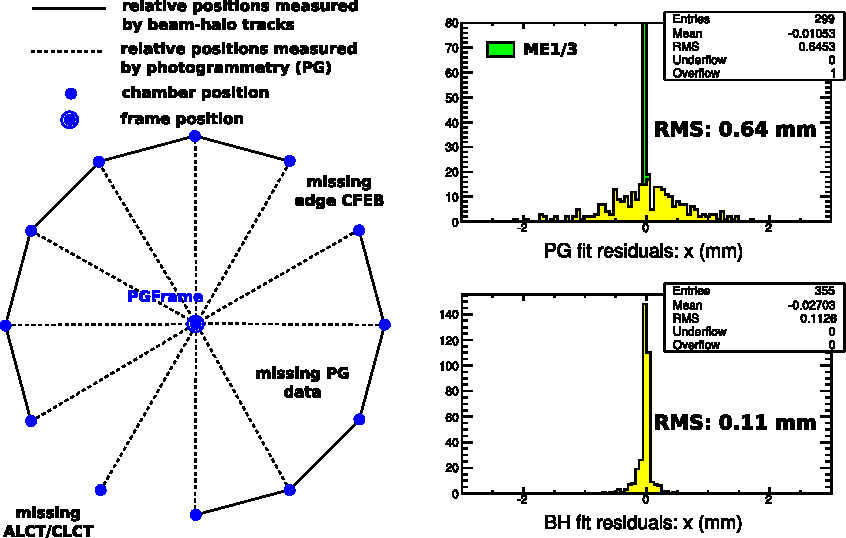
\includegraphics[width=0.9\linewidth]{beamhalo-PG.pdf}
\end{frame}

\begin{frame}
\frametitle{All results: ME$-$1/1 $r\phi$}
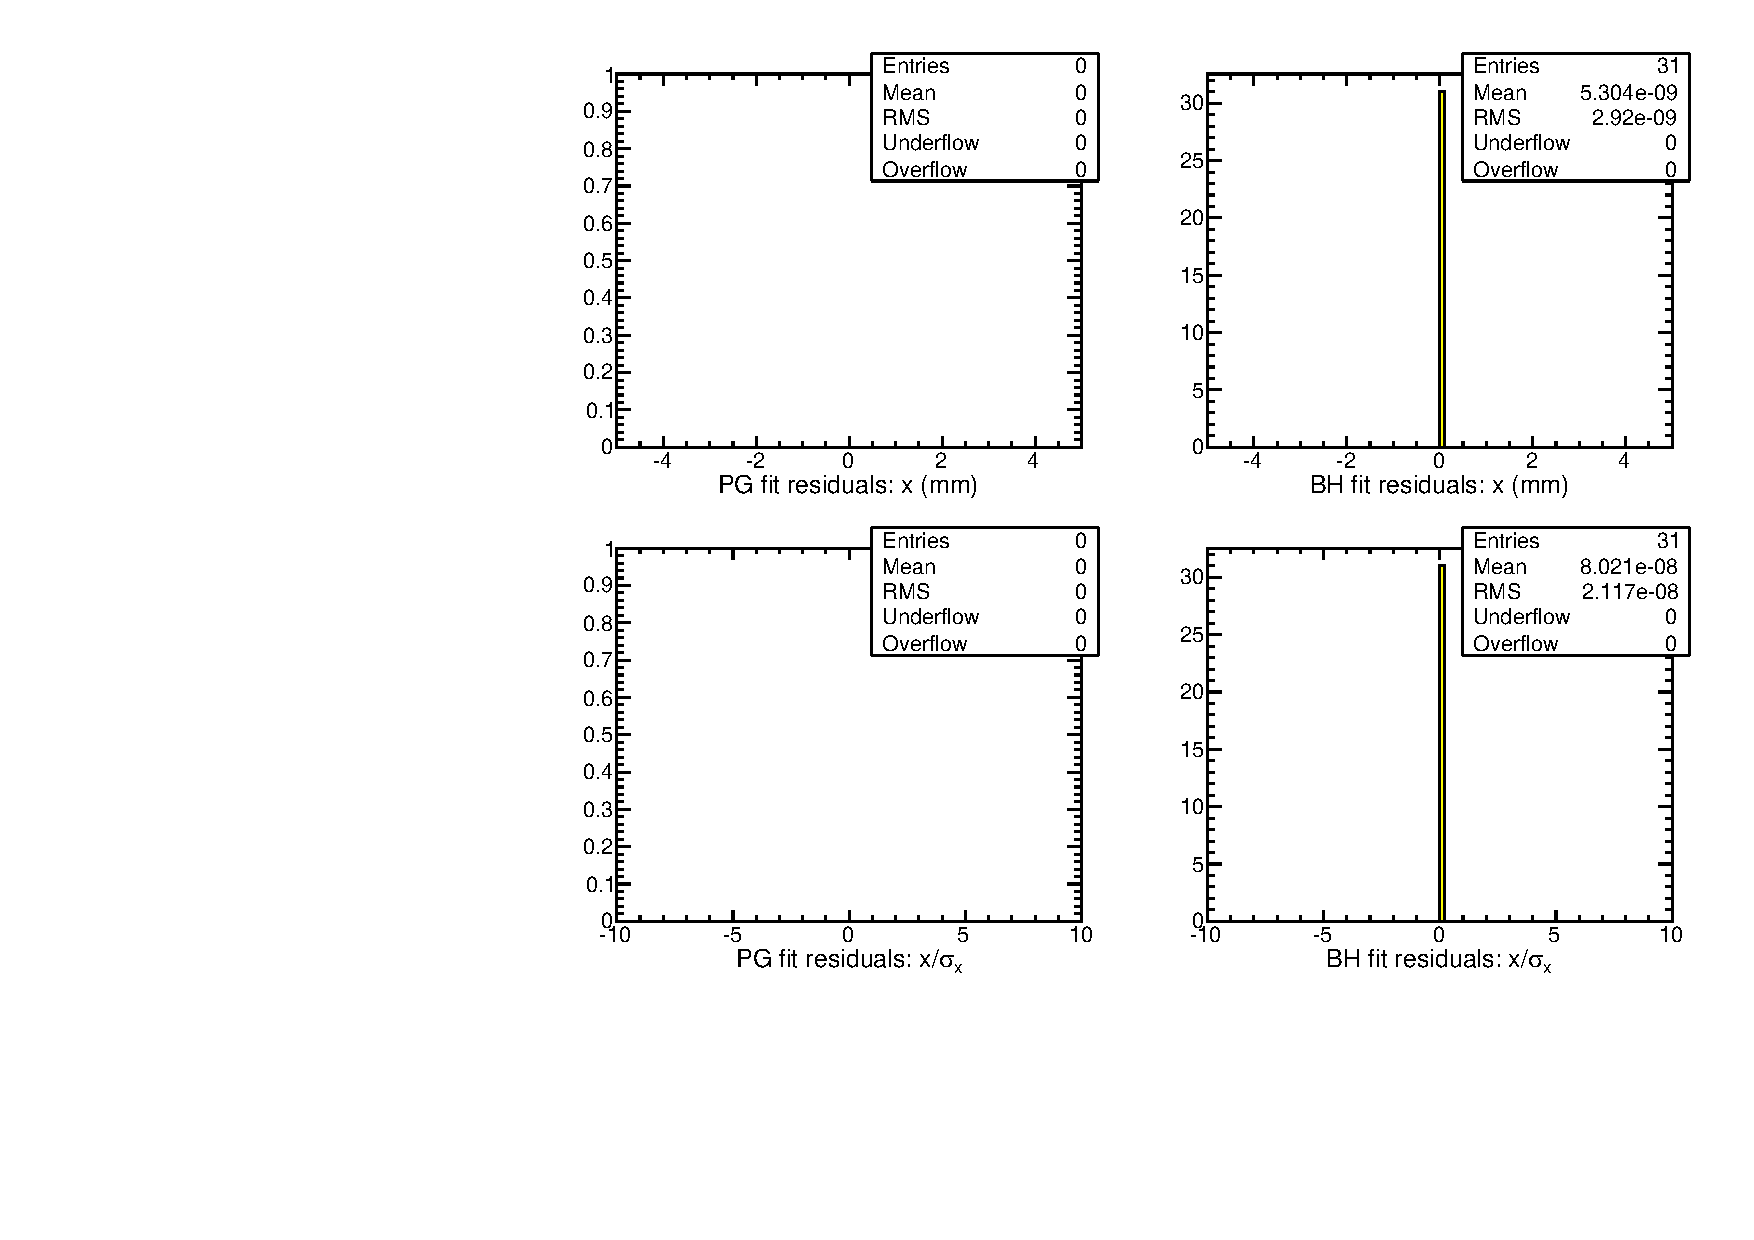
\includegraphics[width=\linewidth]{newplots_fitresiduals_MEm1_1_x.pdf}
\end{frame}
\begin{frame}
\frametitle{All results: ME$-$1/1 $\phi_z$}
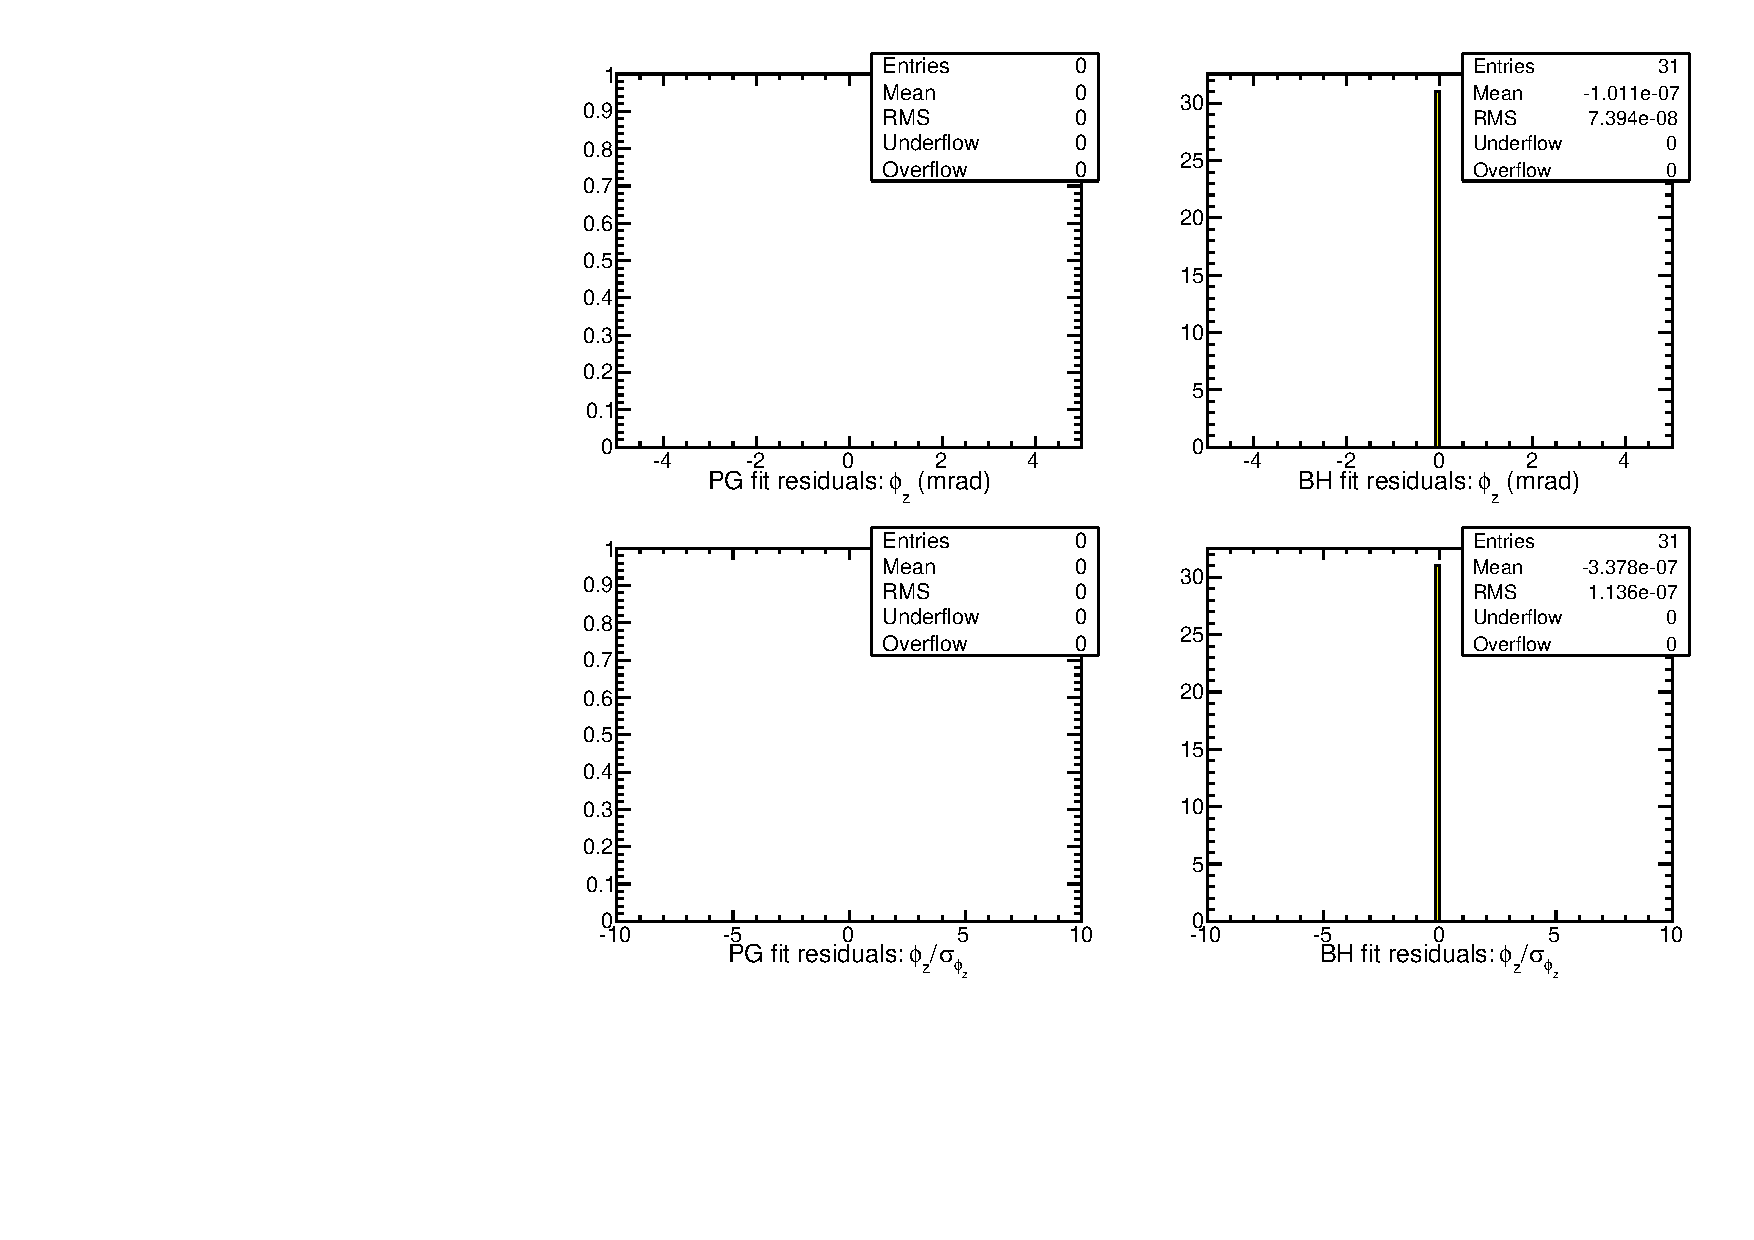
\includegraphics[width=\linewidth]{newplots_fitresiduals_MEm1_1_phiz.pdf}
\end{frame}
\begin{frame}
\frametitle{All results: YE$-$1 $r\phi$}
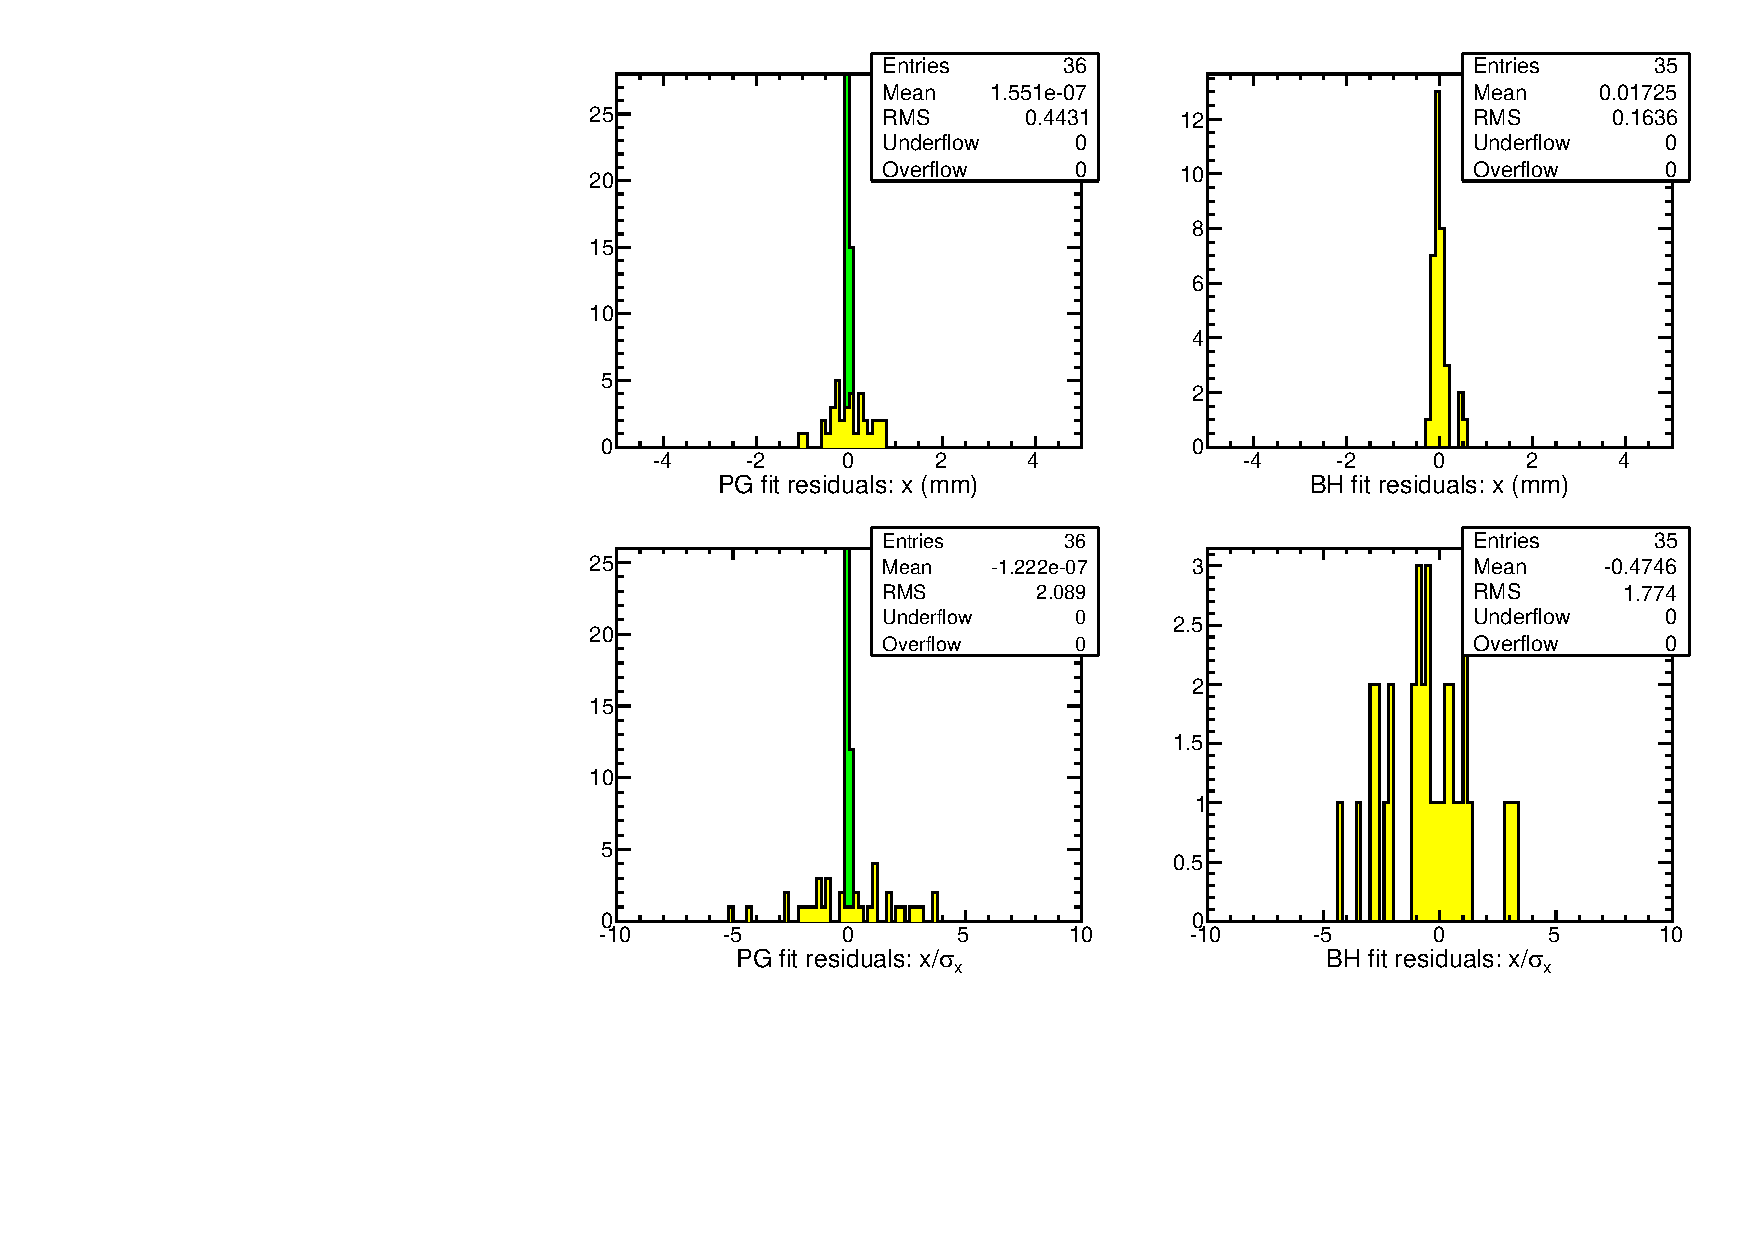
\includegraphics[width=\linewidth]{newplots_fitresiduals_YEm1_x.pdf}
\end{frame}
\begin{frame}
\frametitle{All results: YE$-$1 $\phi_z$}
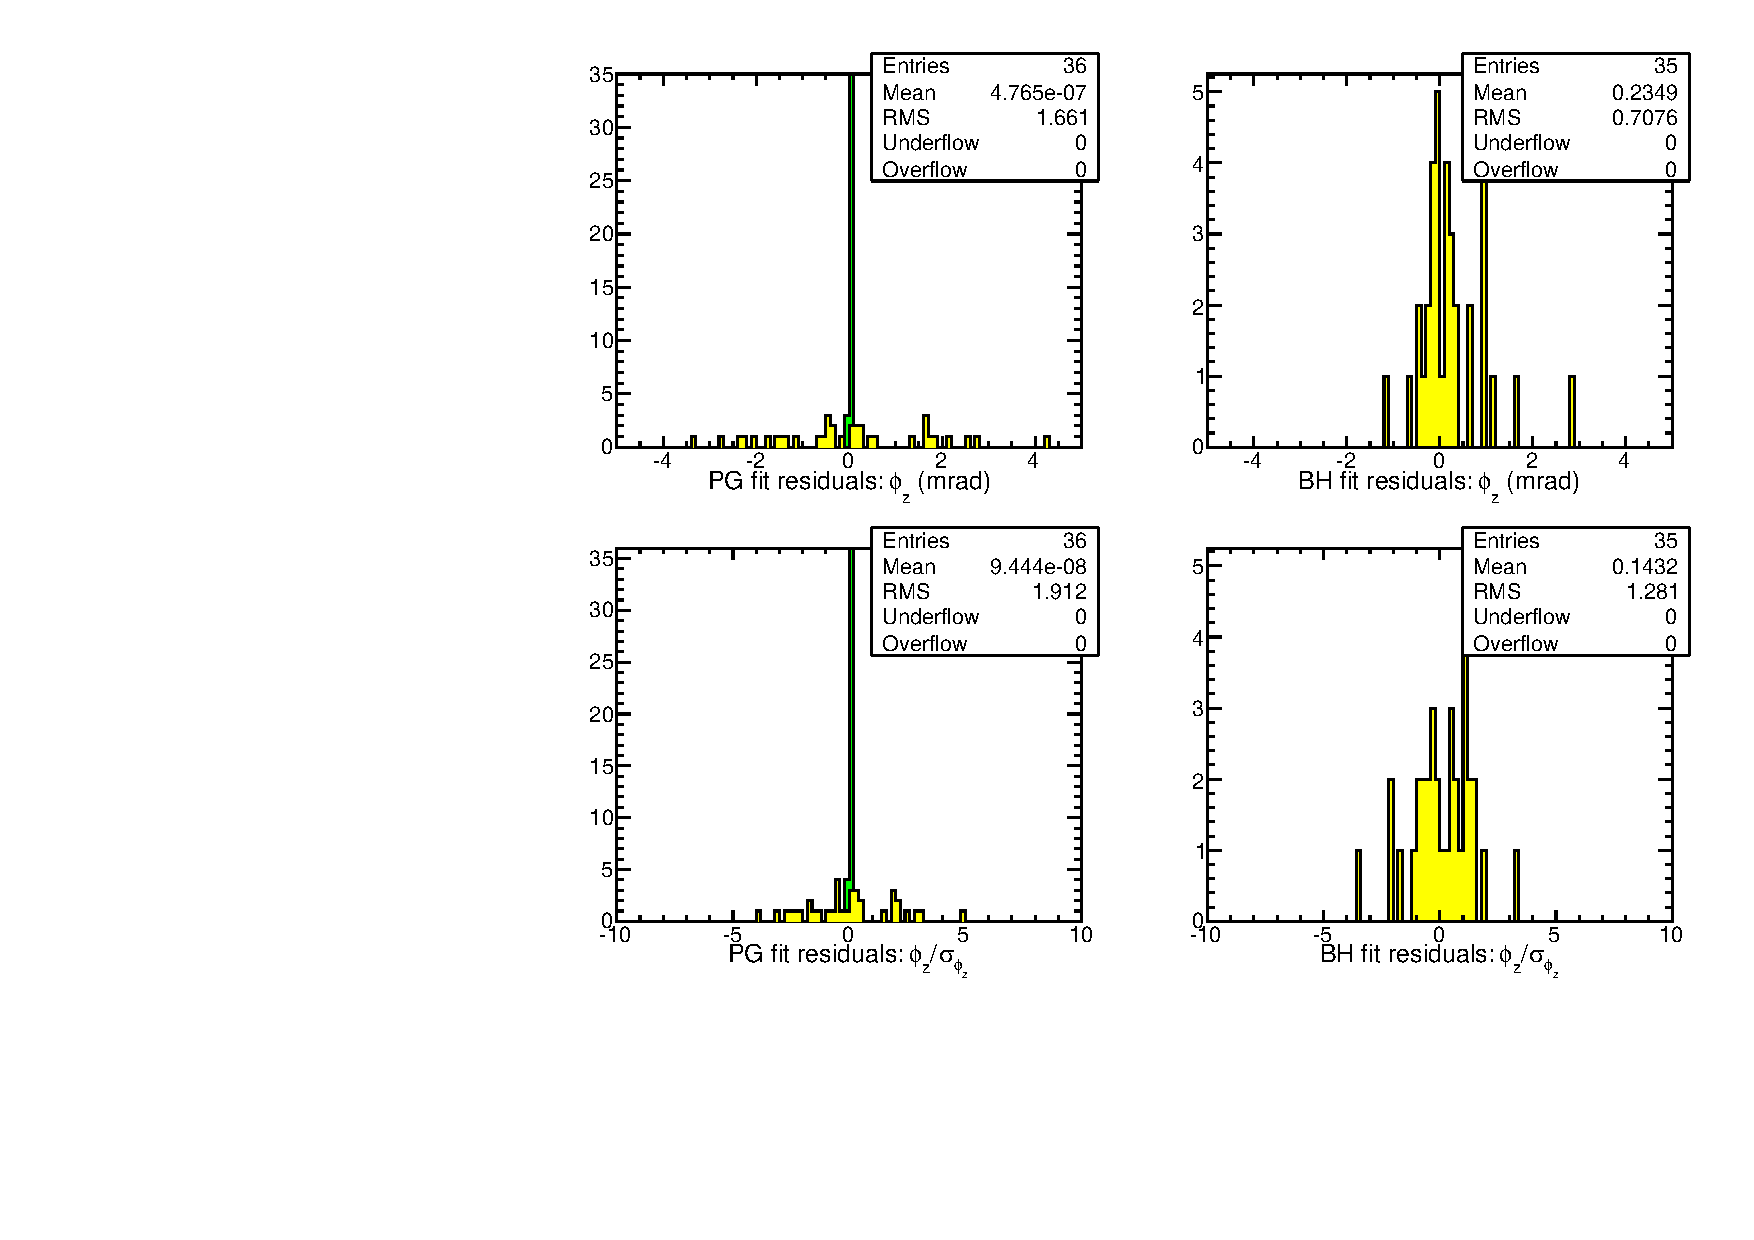
\includegraphics[width=\linewidth]{newplots_fitresiduals_YEm1_phiz.pdf}
\end{frame}
\begin{frame}
\frametitle{All results: YE$-$2 $r\phi$}
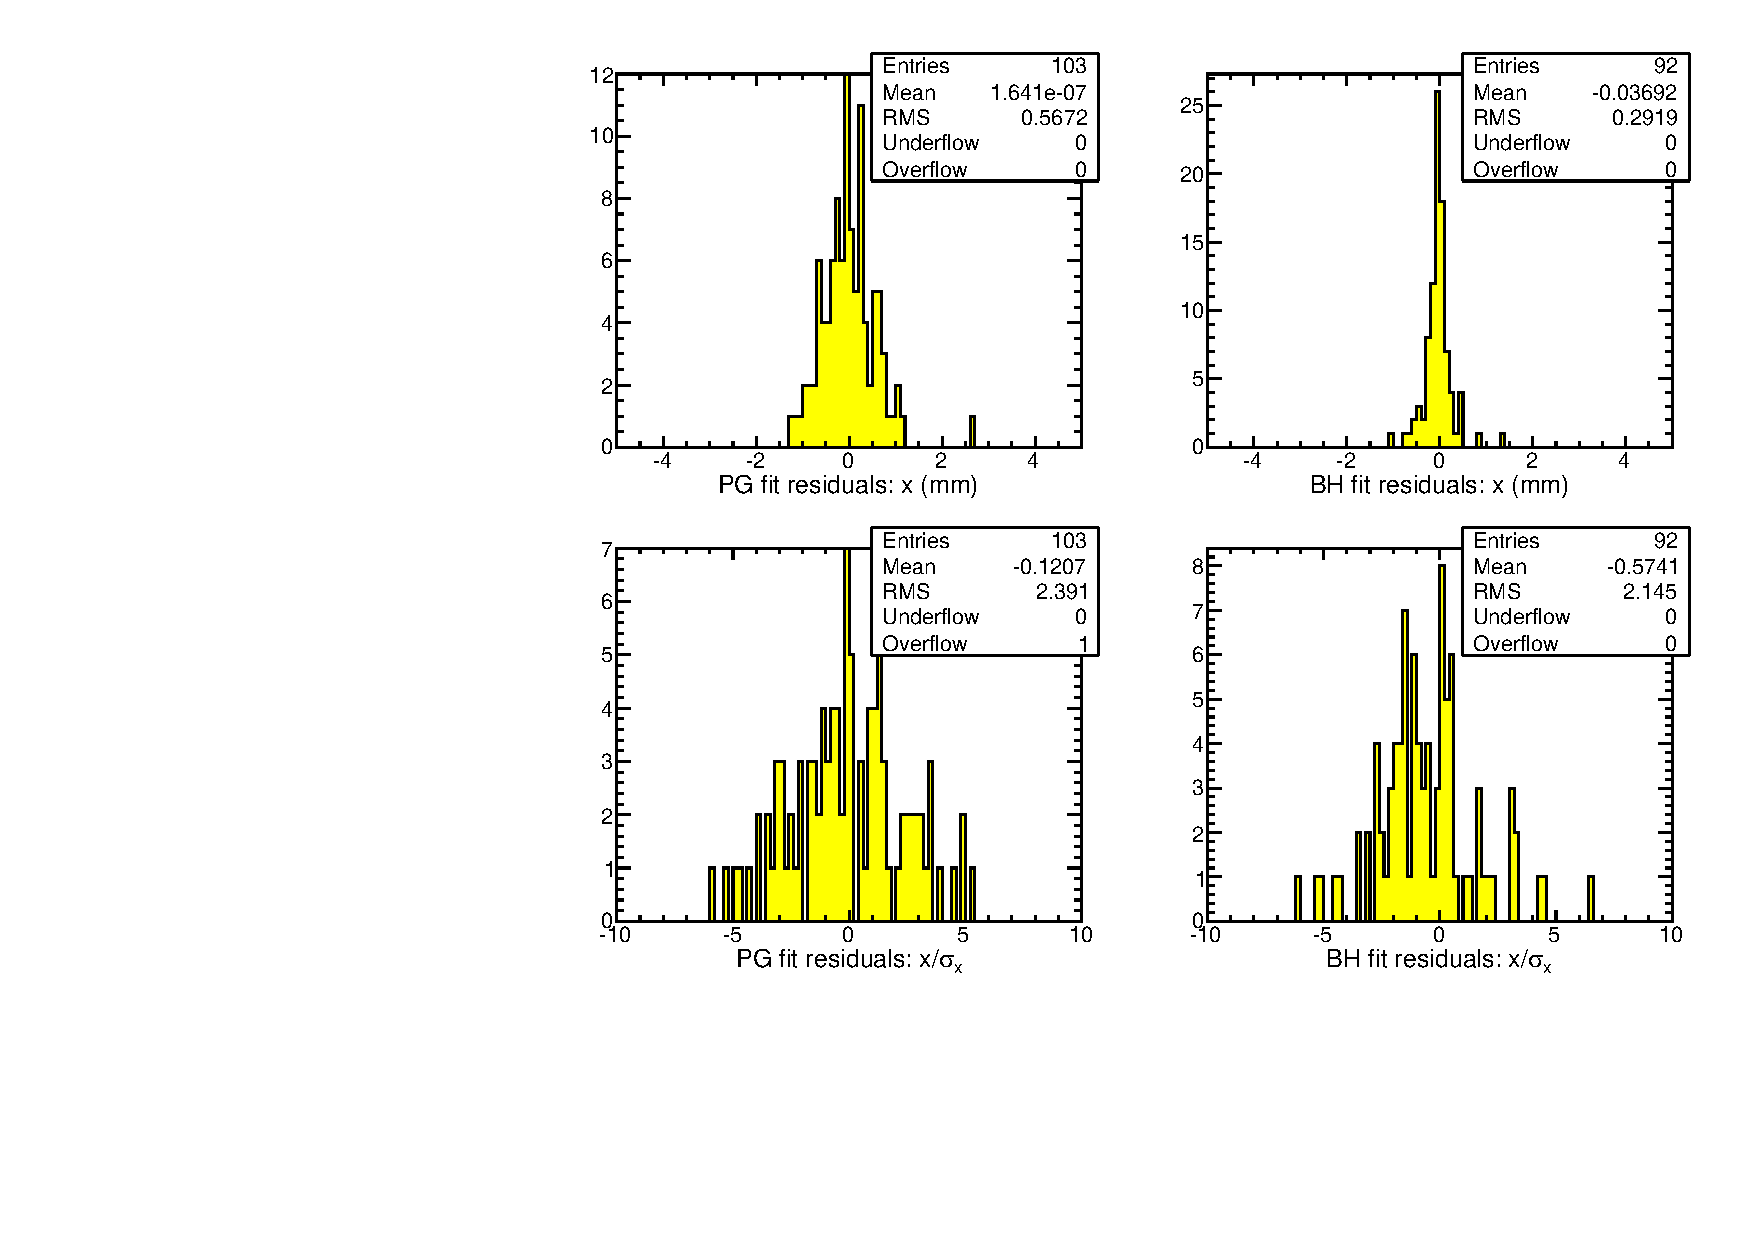
\includegraphics[width=\linewidth]{newplots_fitresiduals_YEm2_x.pdf}
\end{frame}
\begin{frame}
\frametitle{All results: YE$-$2 $\phi_z$}
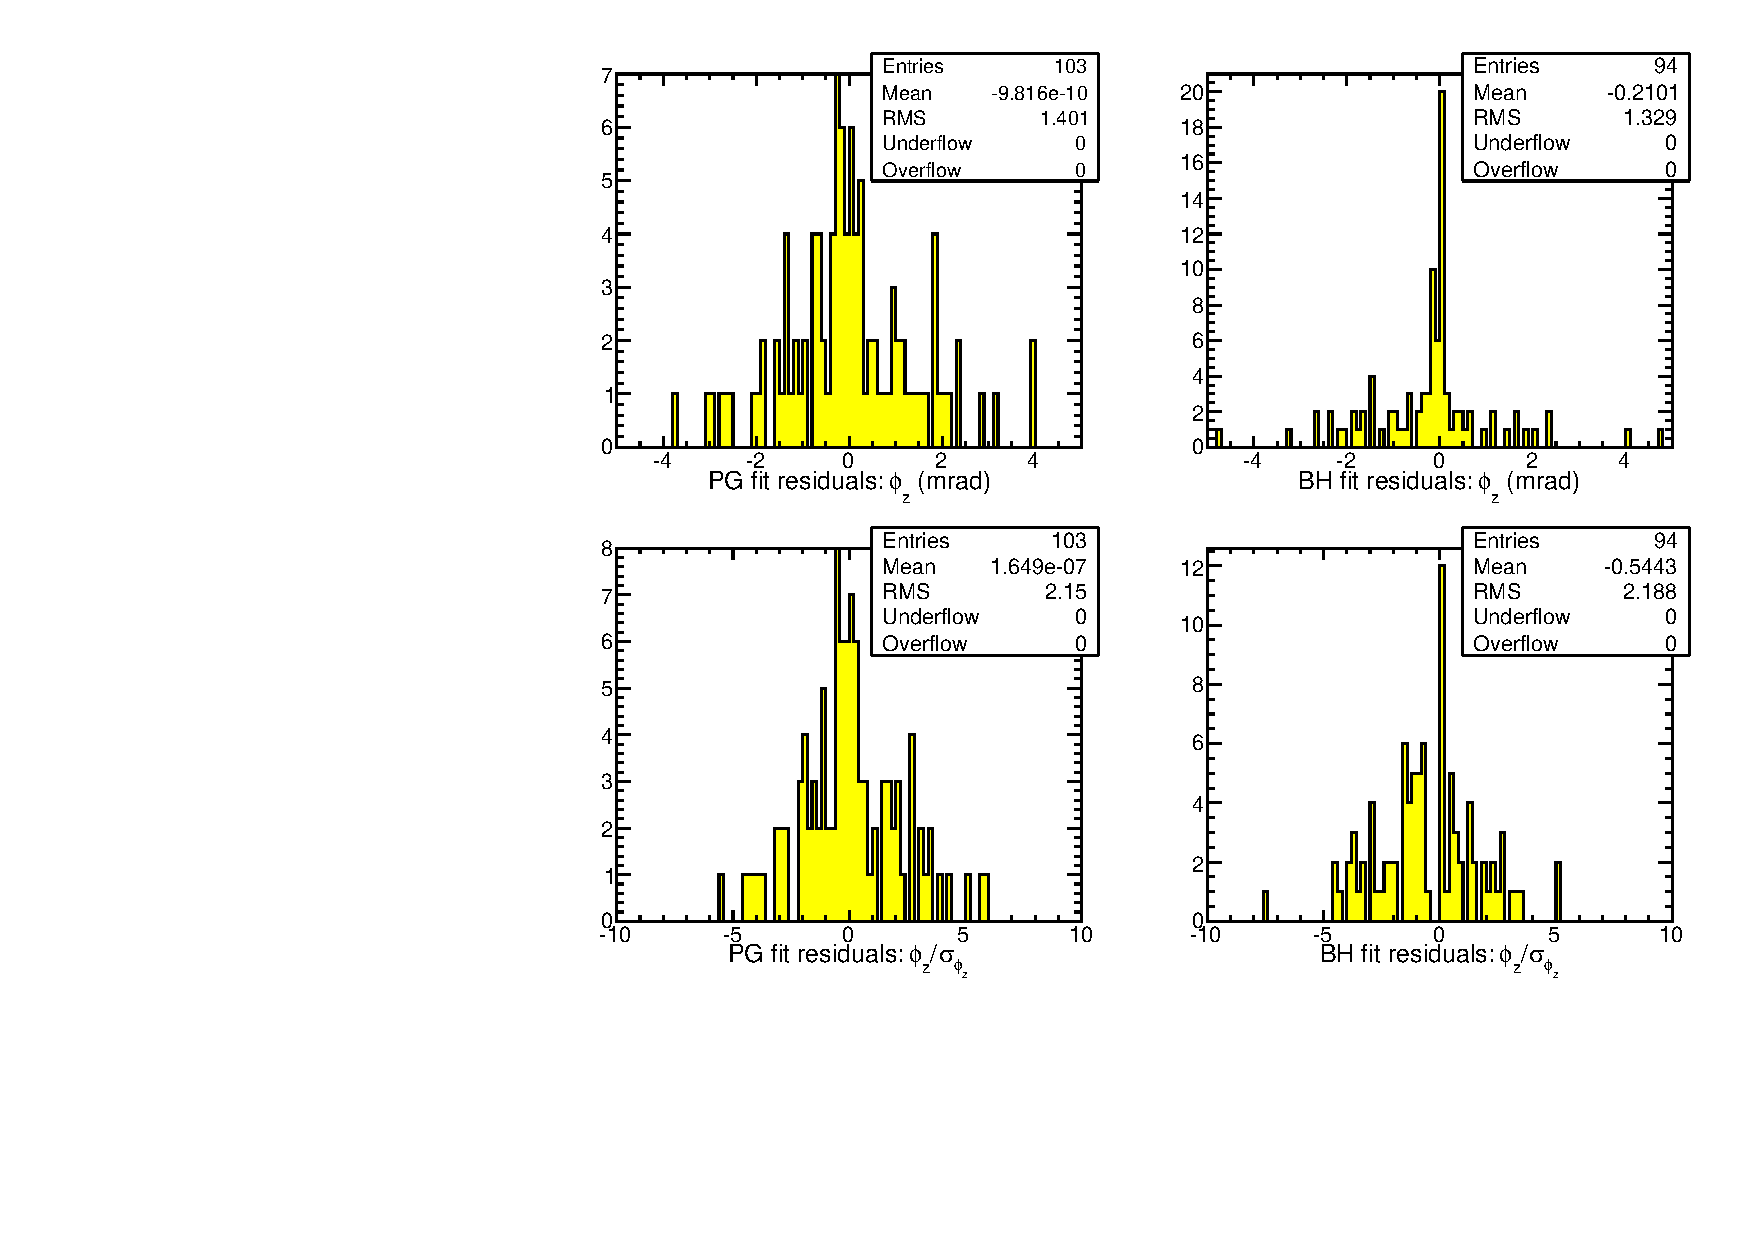
\includegraphics[width=\linewidth]{newplots_fitresiduals_YEm2_phiz.pdf}
\end{frame}
\begin{frame}
\frametitle{All results: ME$-$4/1 $r\phi$}
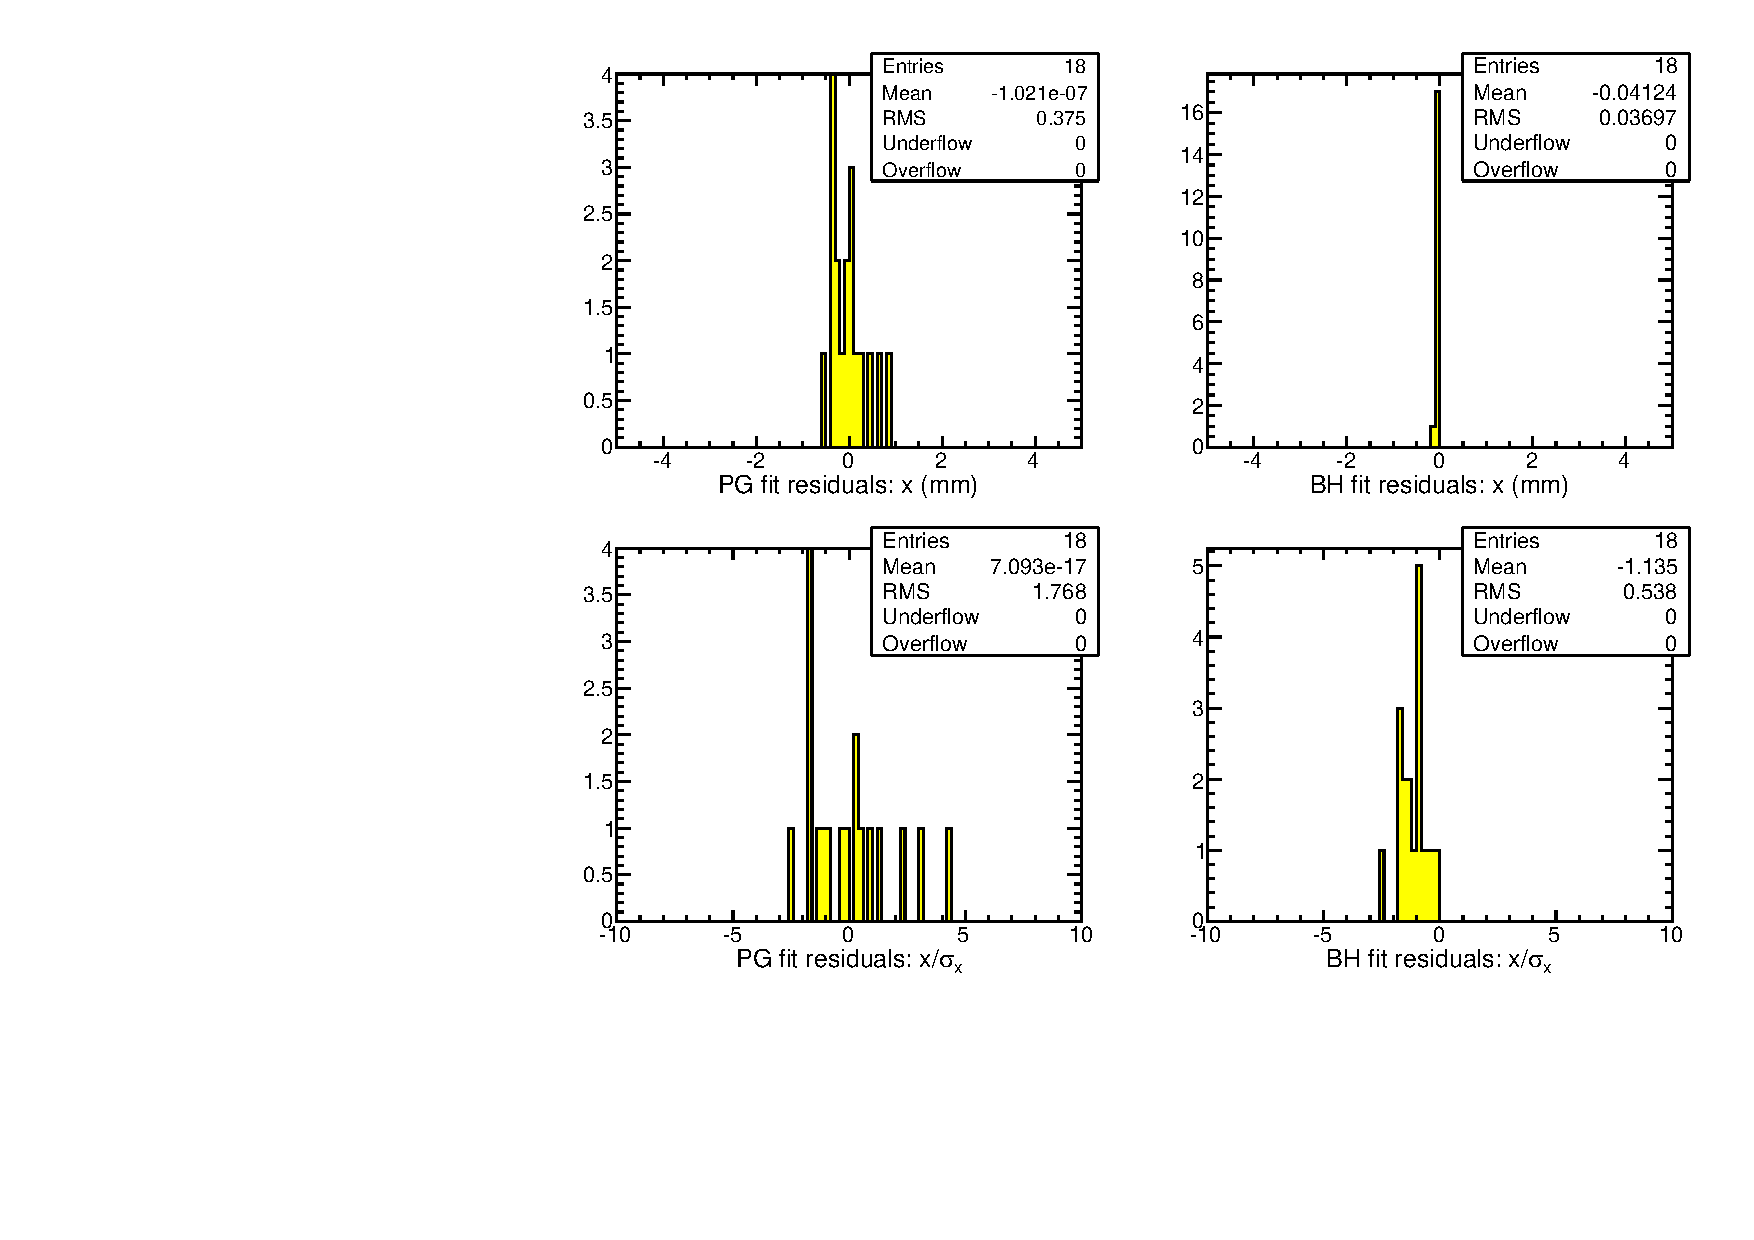
\includegraphics[width=\linewidth]{newplots_fitresiduals_MEm4_1_x.pdf}
\end{frame}
\begin{frame}
\frametitle{All results: ME$-$4/1 $\phi_z$}
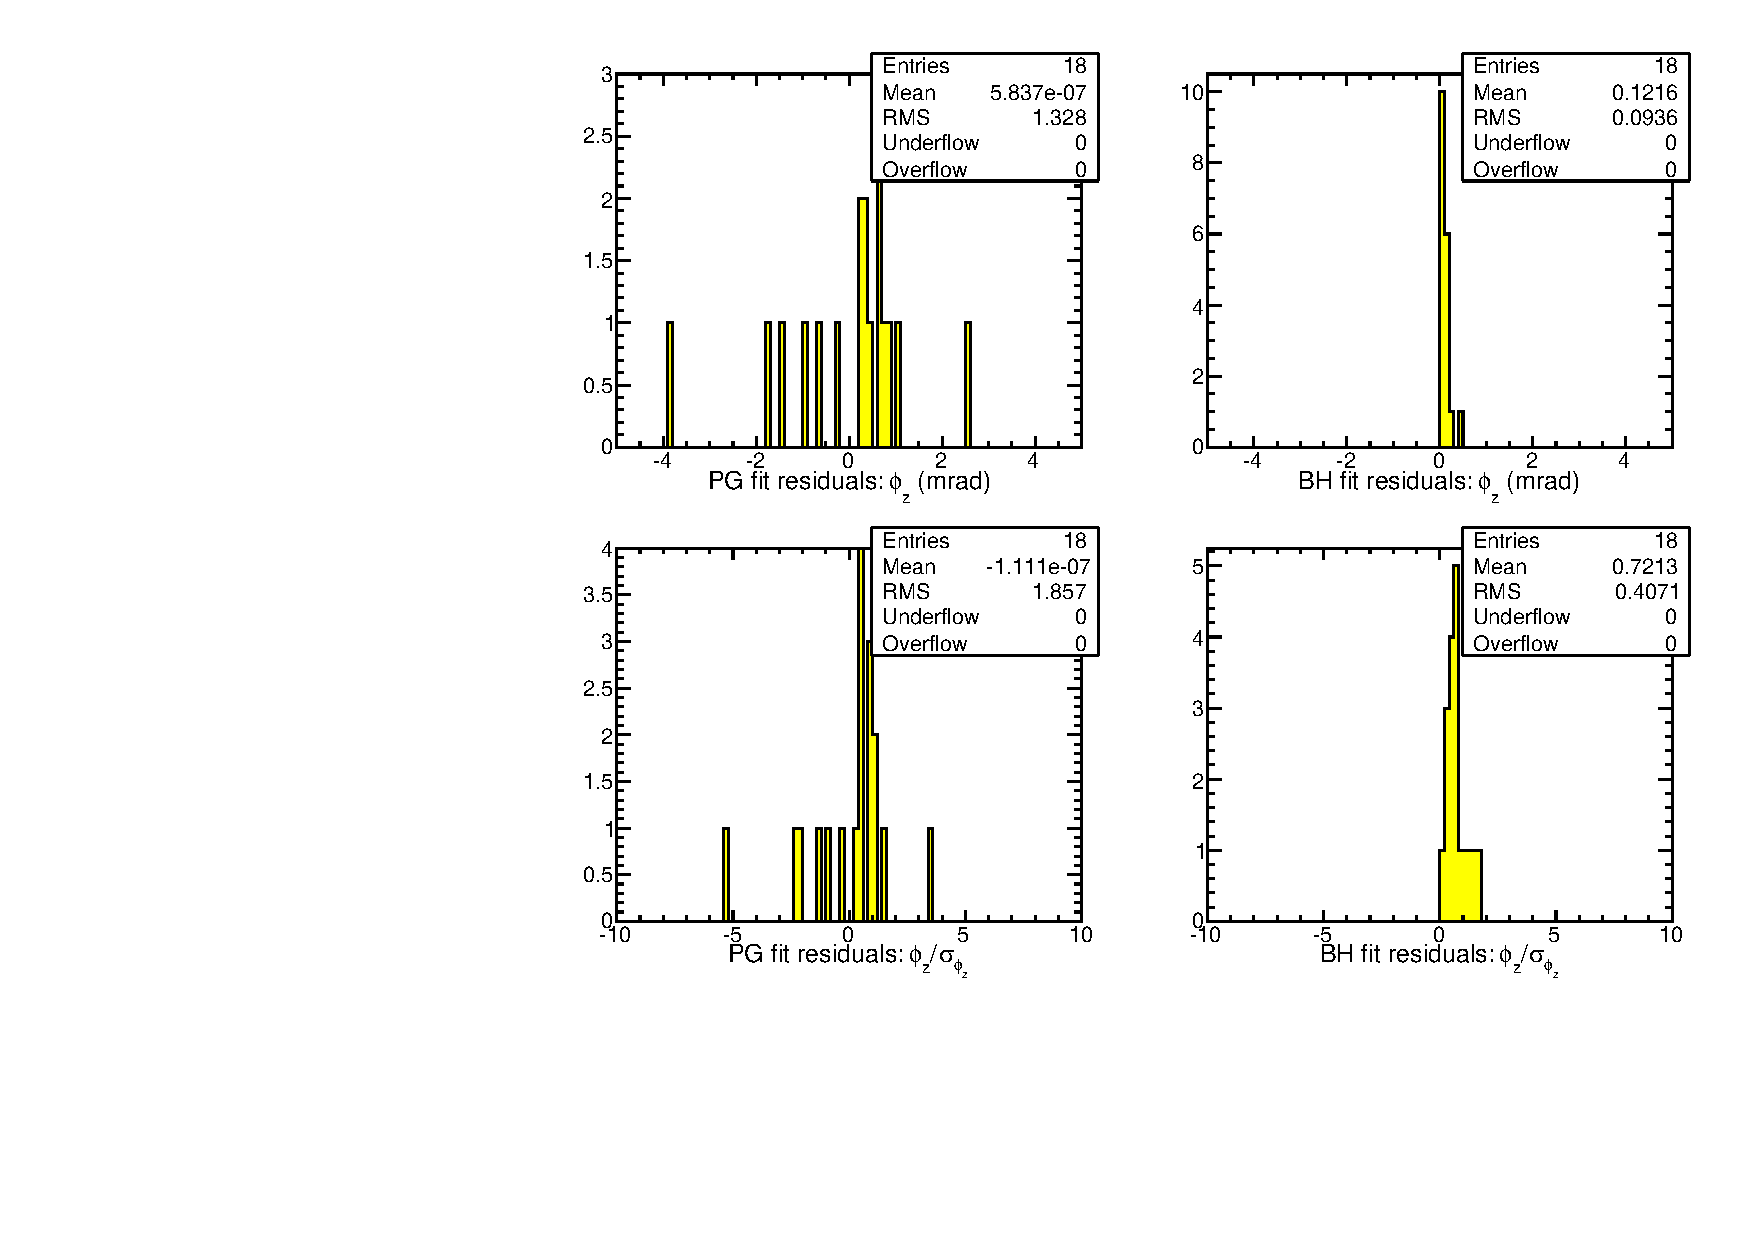
\includegraphics[width=\linewidth]{newplots_fitresiduals_MEm4_1_phiz.pdf}
\end{frame}
\begin{frame}
\frametitle{All results: ME$+$1/1 $r\phi$}
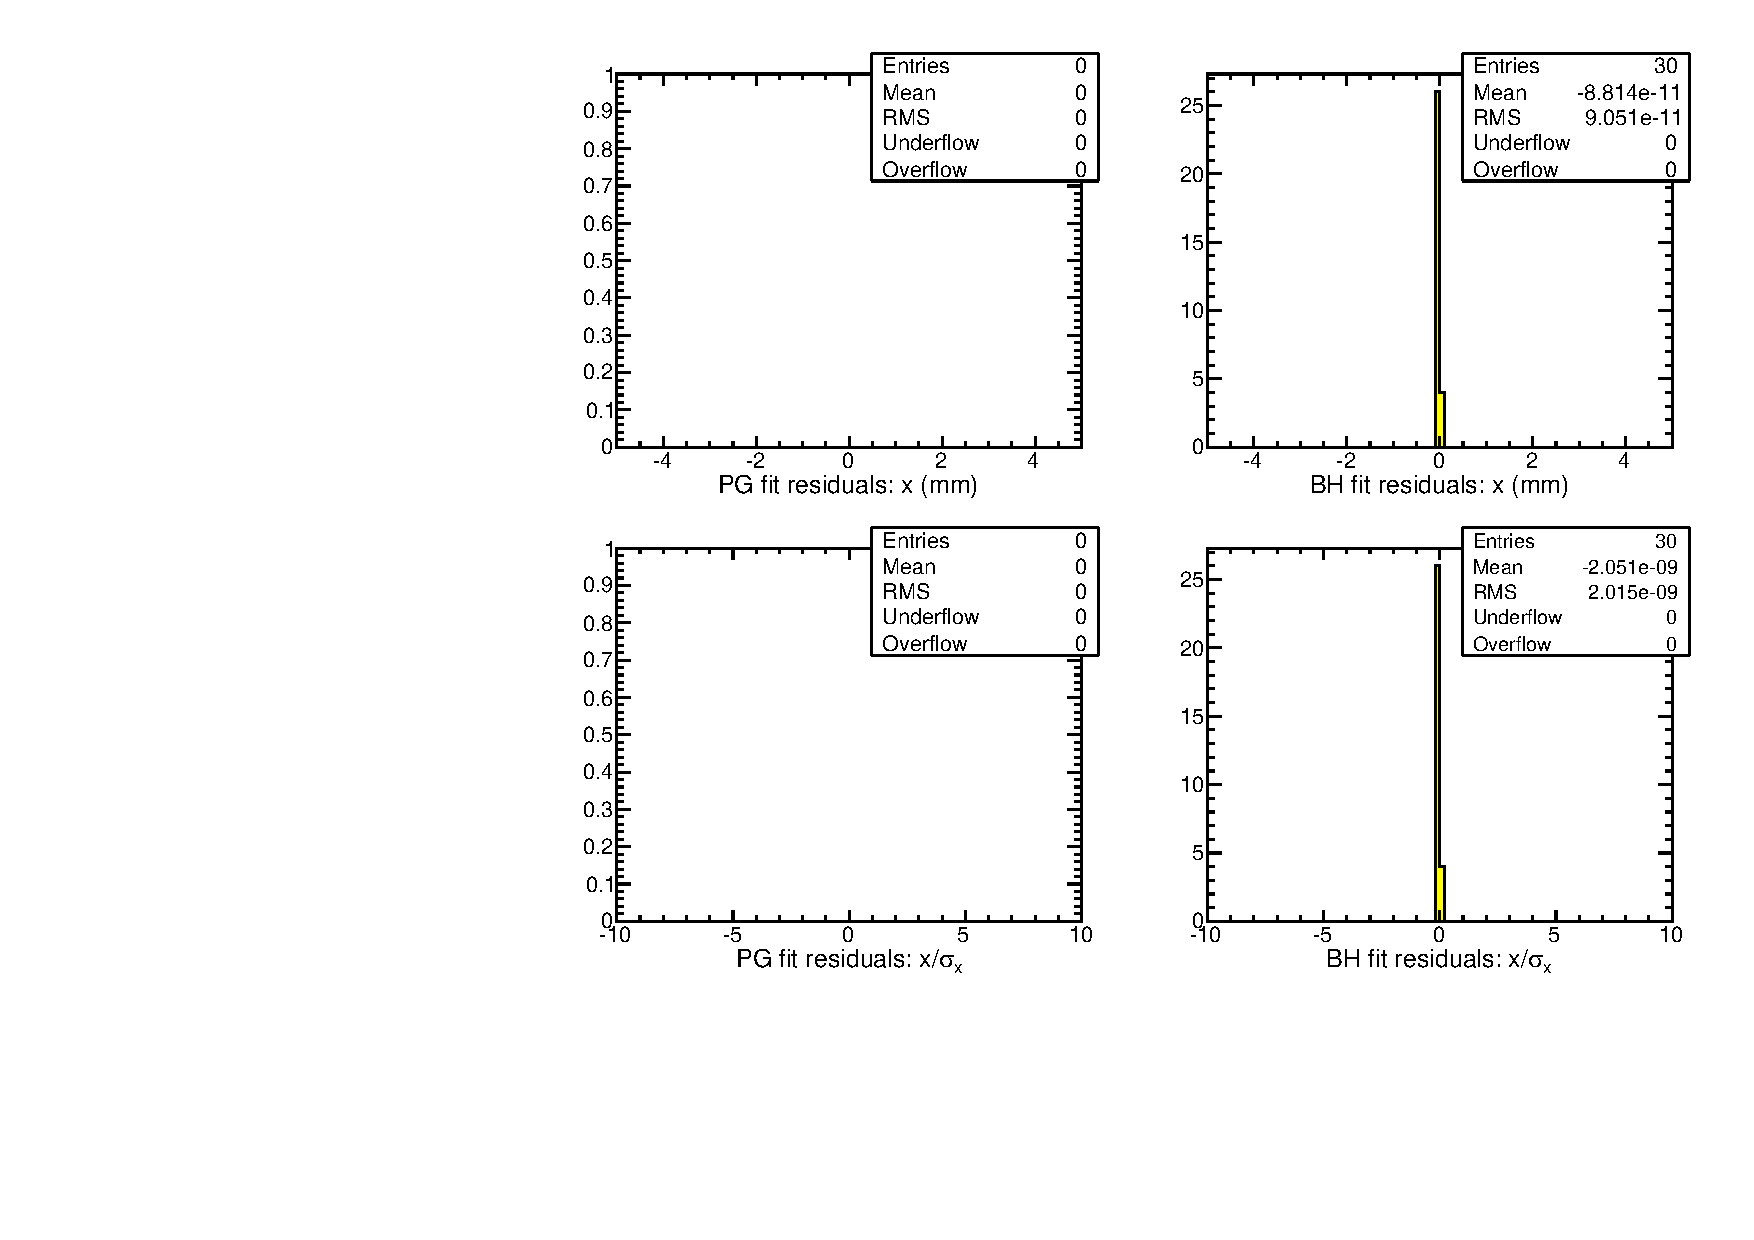
\includegraphics[width=\linewidth]{newplots_fitresiduals_MEp1_1_x.pdf}
\end{frame}
\begin{frame}
\frametitle{All results: ME$+$1/1 $\phi_z$}
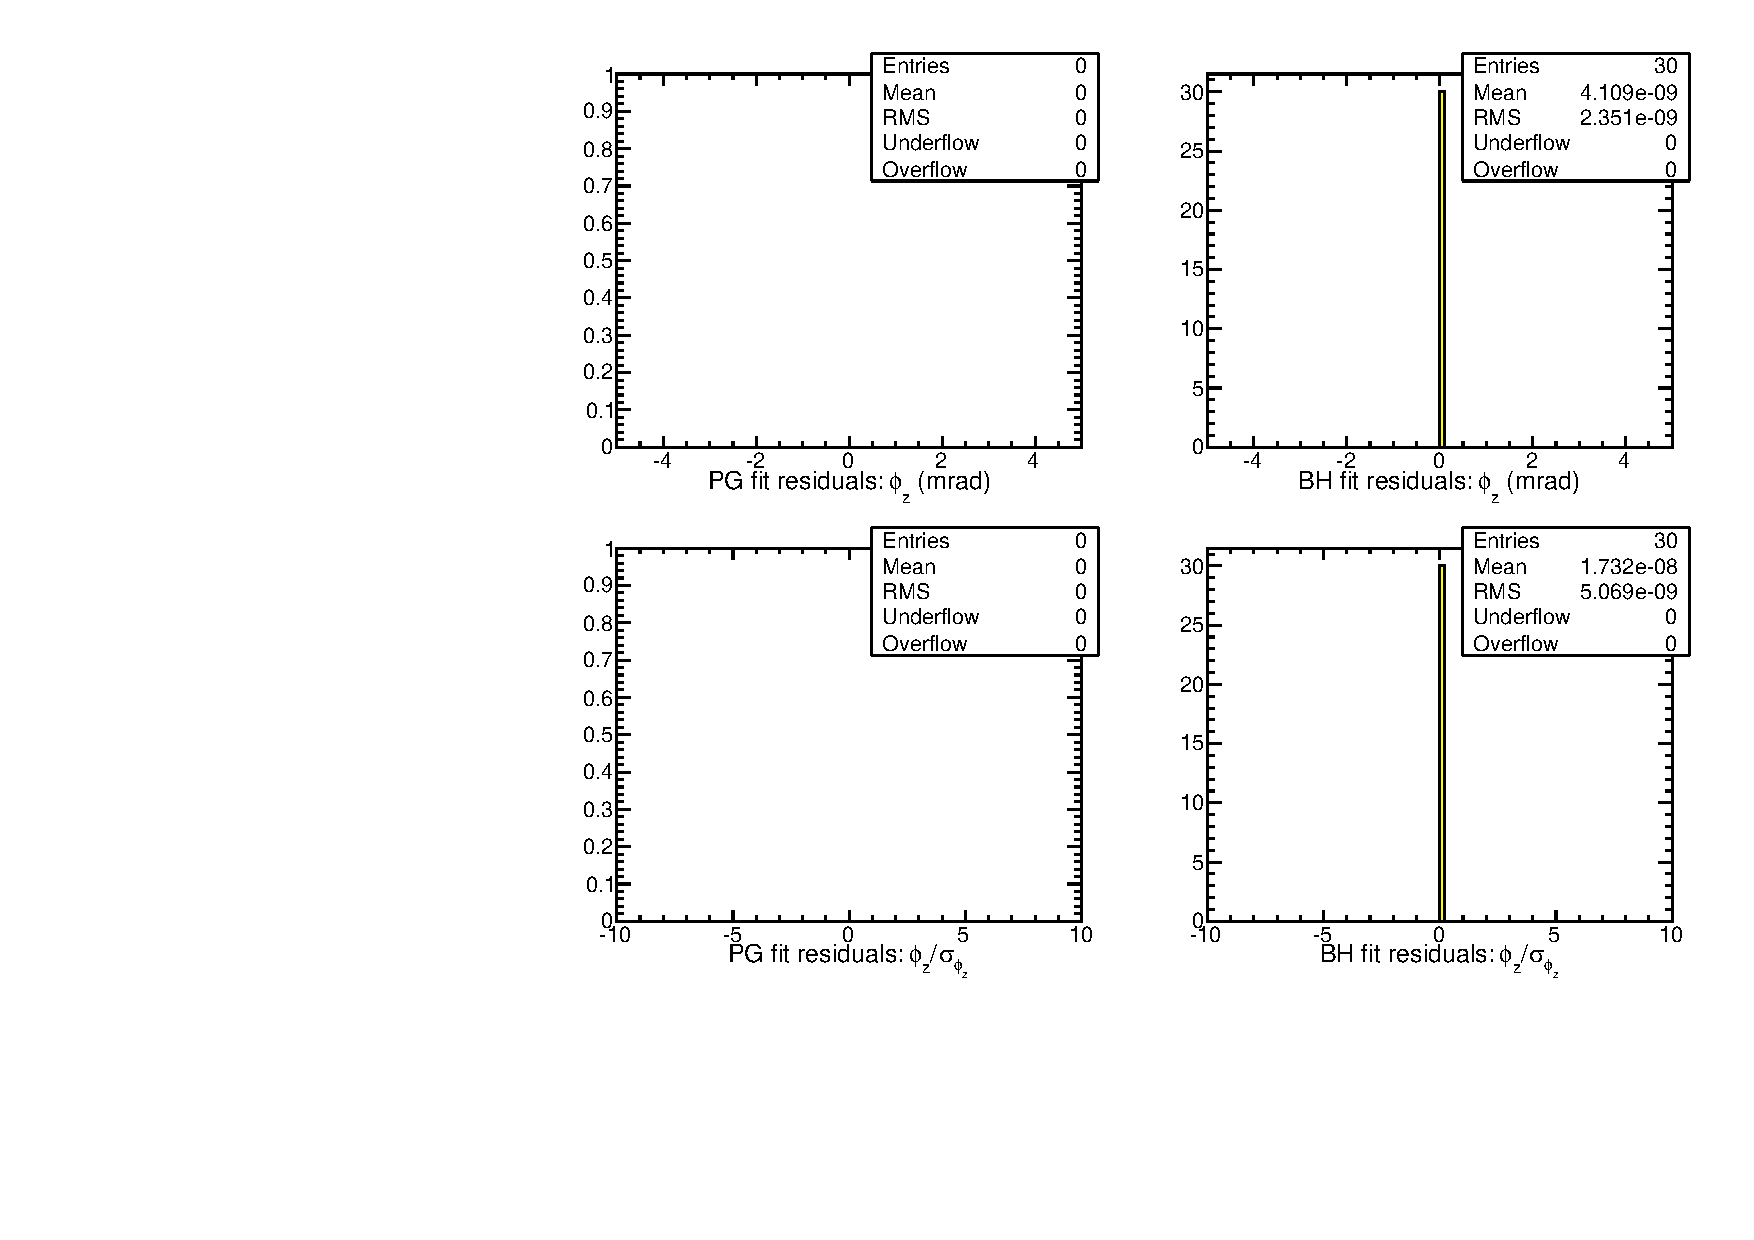
\includegraphics[width=\linewidth]{newplots_fitresiduals_MEp1_1_phiz.pdf}
\end{frame}
\begin{frame}
\frametitle{All results: YE$+$1 $r\phi$}
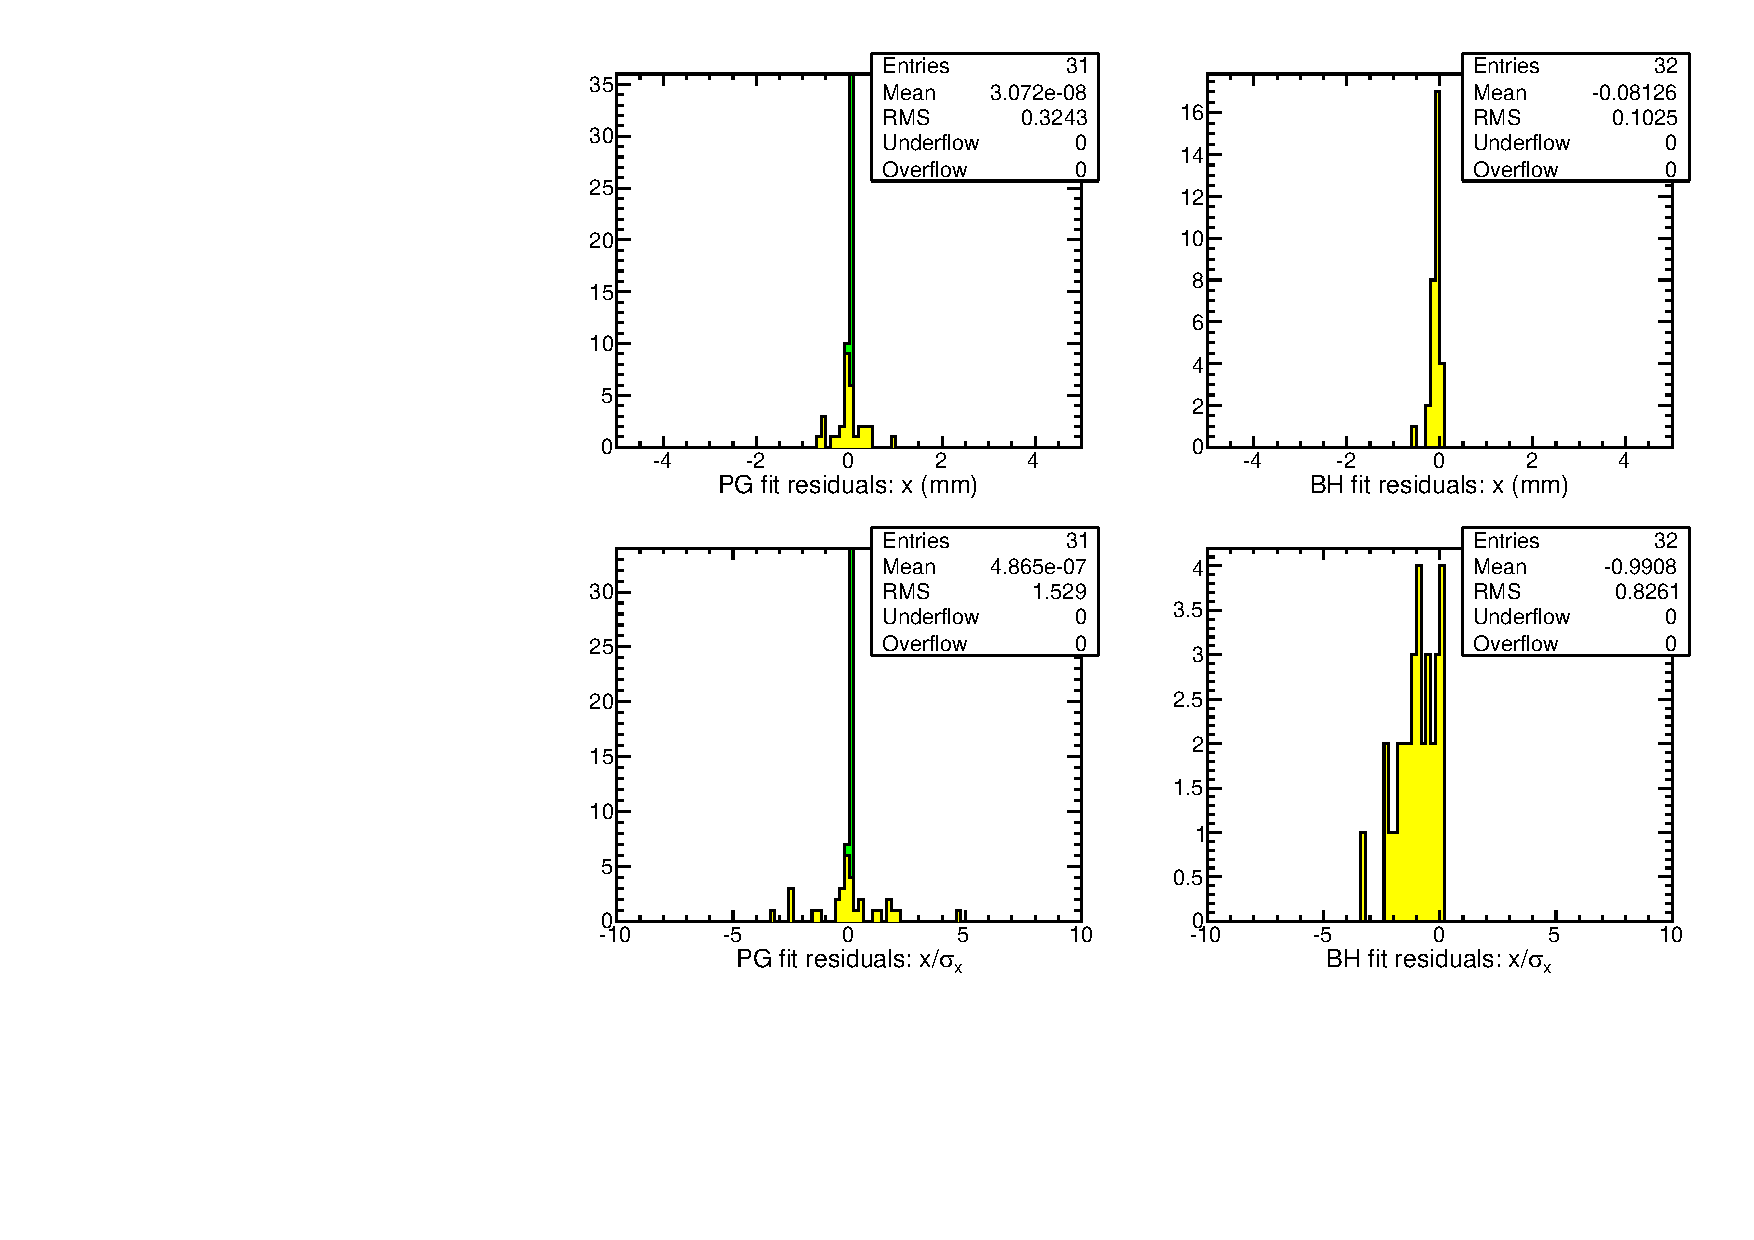
\includegraphics[width=\linewidth]{newplots_fitresiduals_YEp1_x.pdf}
\end{frame}
\begin{frame}
\frametitle{All results: YE$+$1 $\phi_z$}
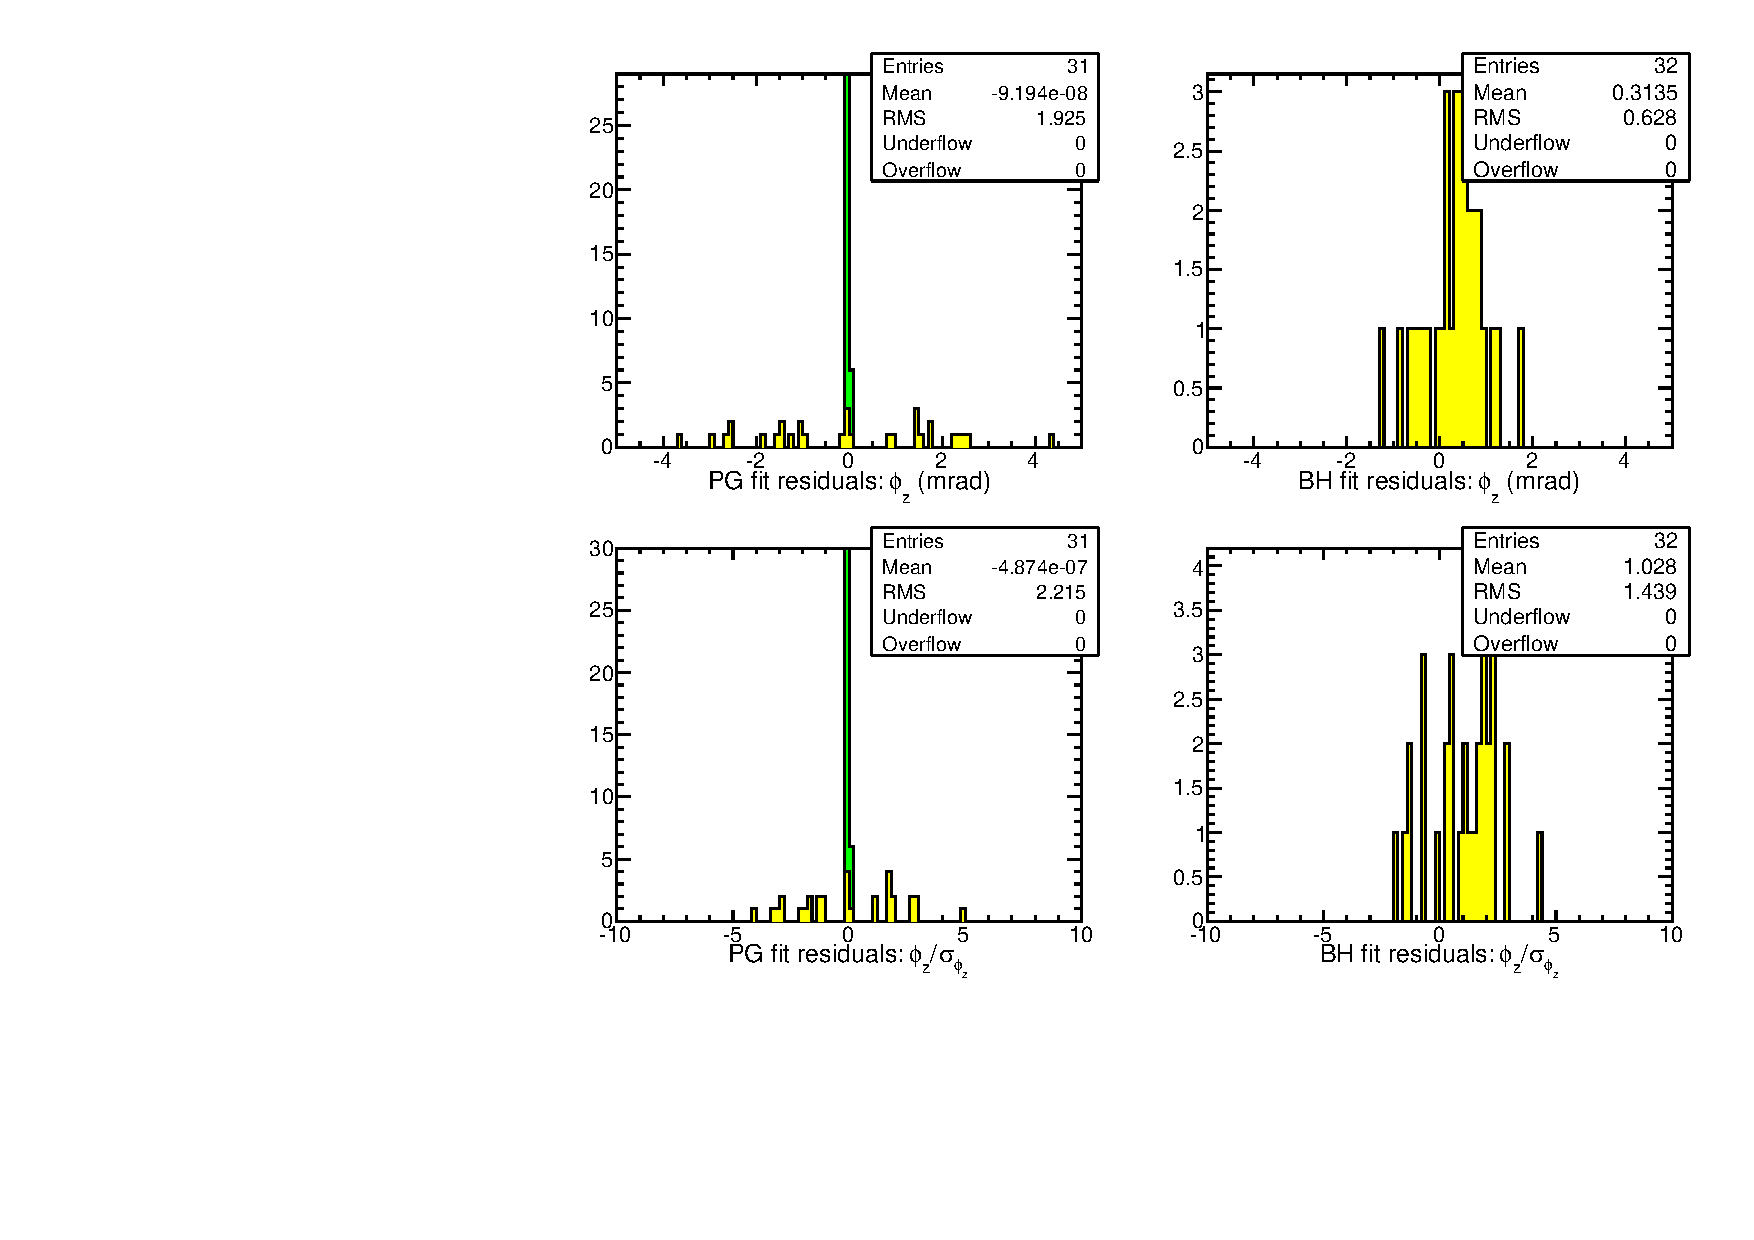
\includegraphics[width=\linewidth]{newplots_fitresiduals_YEp1_phiz.pdf}
\end{frame}
\begin{frame}
\frametitle{All results: YE$+$2 $r\phi$}
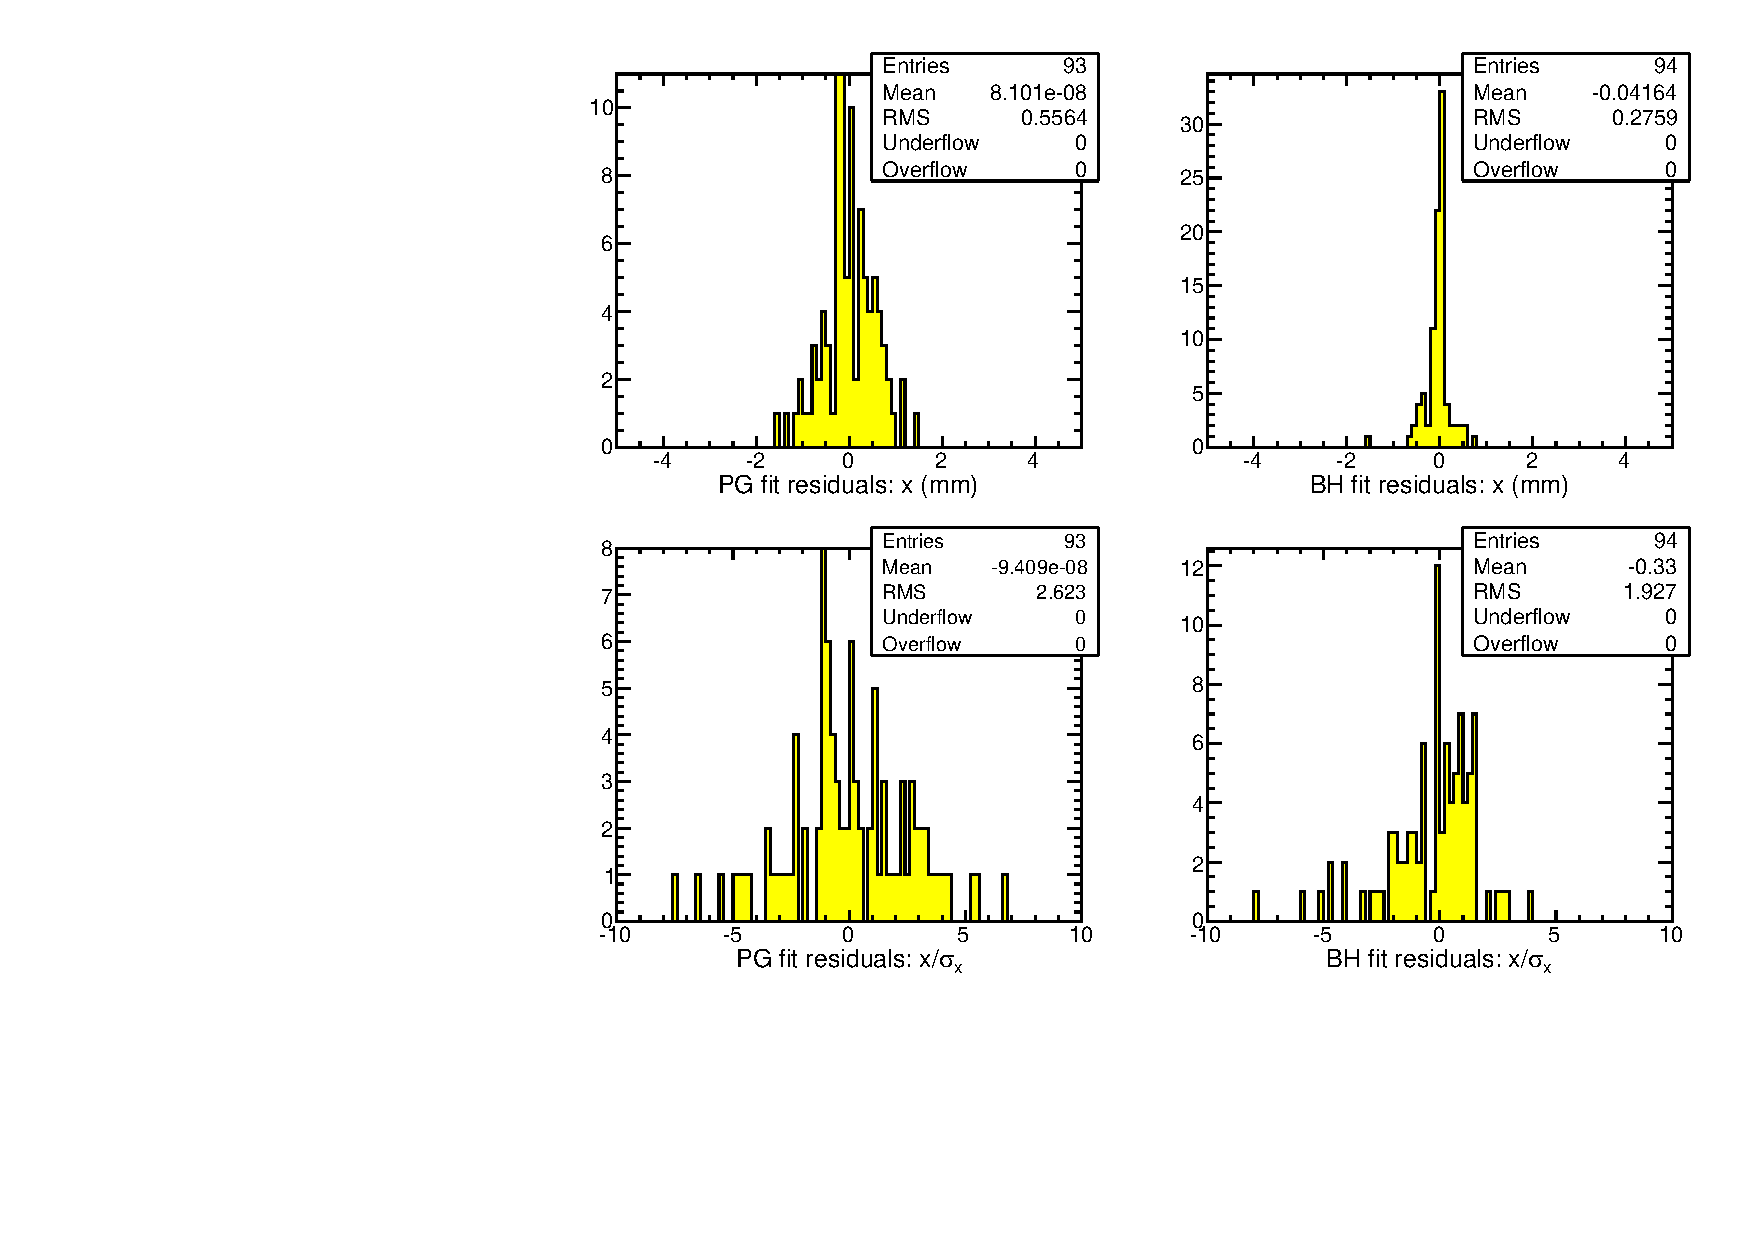
\includegraphics[width=\linewidth]{newplots_fitresiduals_YEp2_x.pdf}
\end{frame}
\begin{frame}
\frametitle{All results: YE$+$2 $\phi_z$}
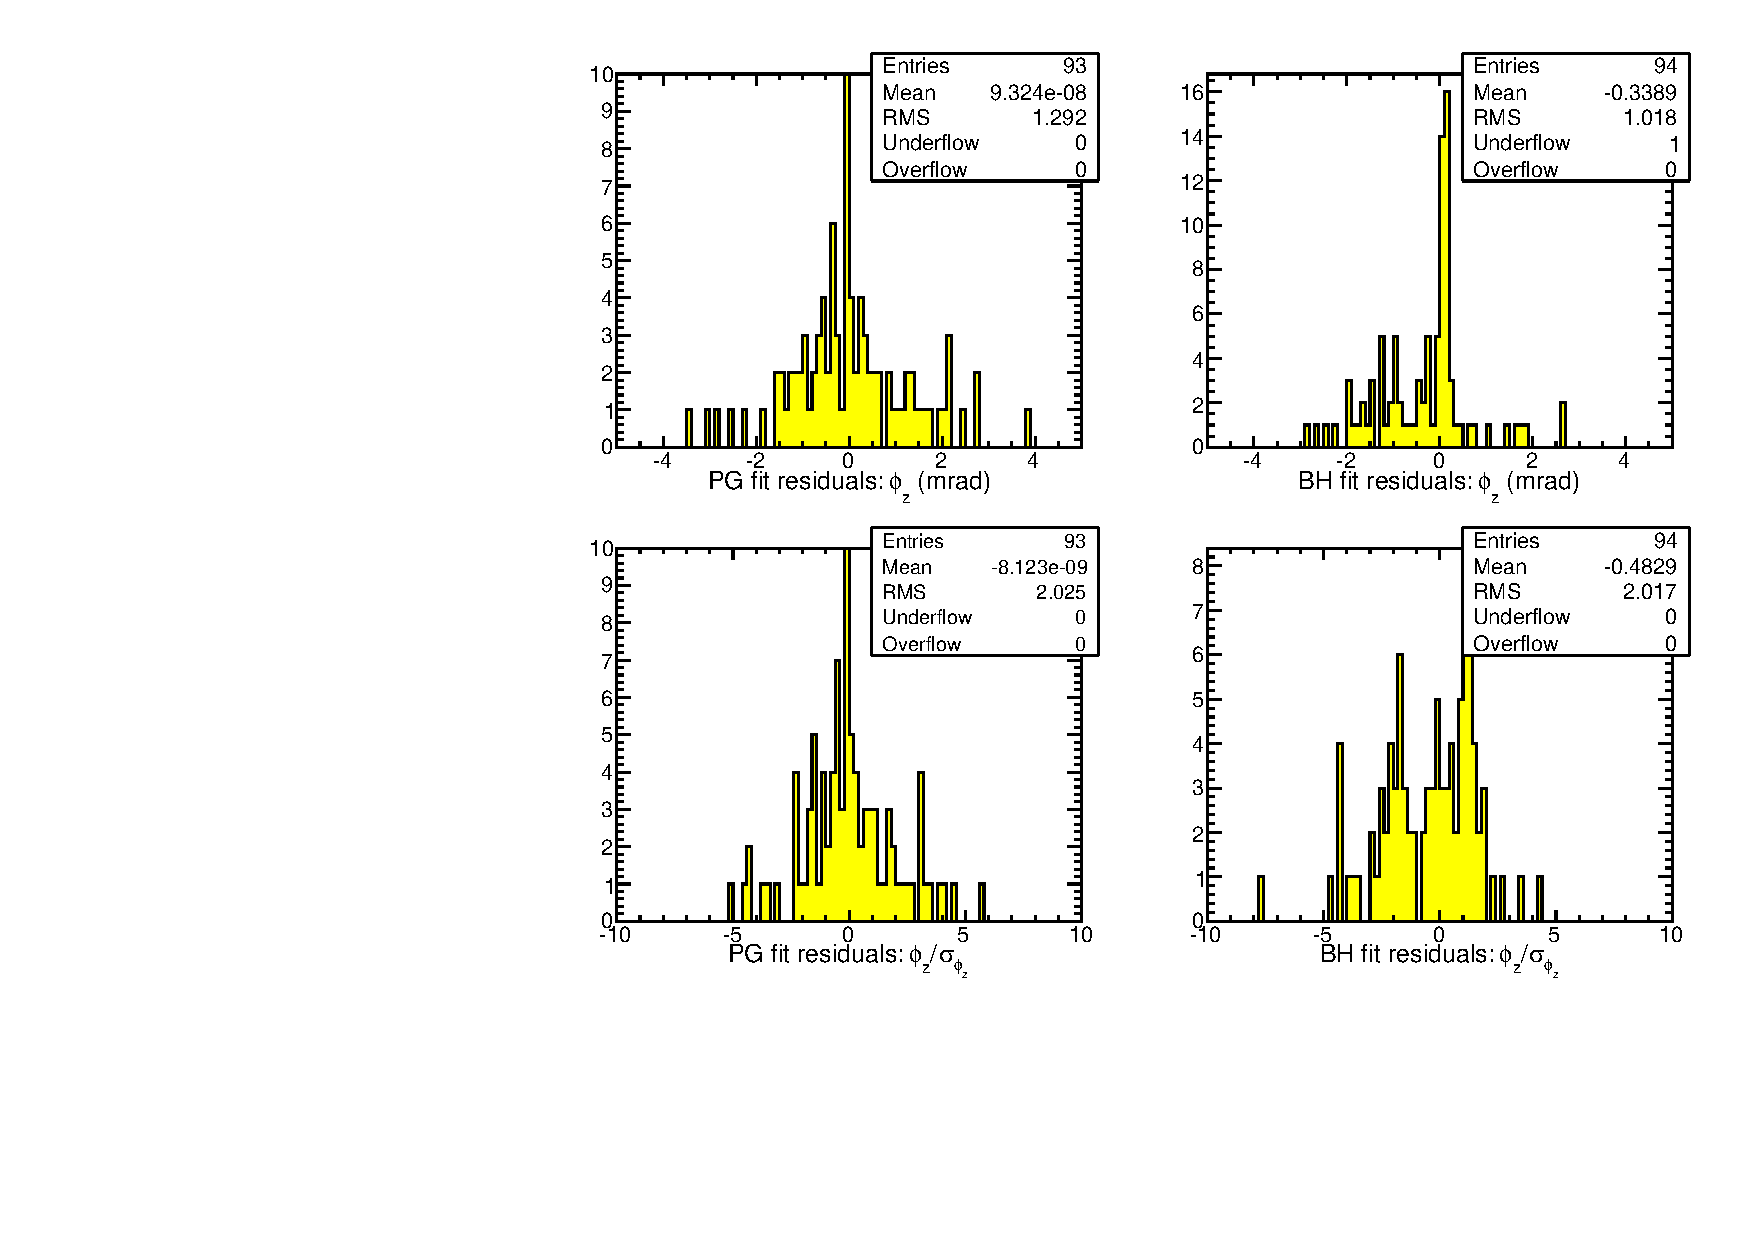
\includegraphics[width=\linewidth]{newplots_fitresiduals_YEp2_phiz.pdf}
\end{frame}
\begin{frame}
\frametitle{All results: ME$+$4/1 $r\phi$}
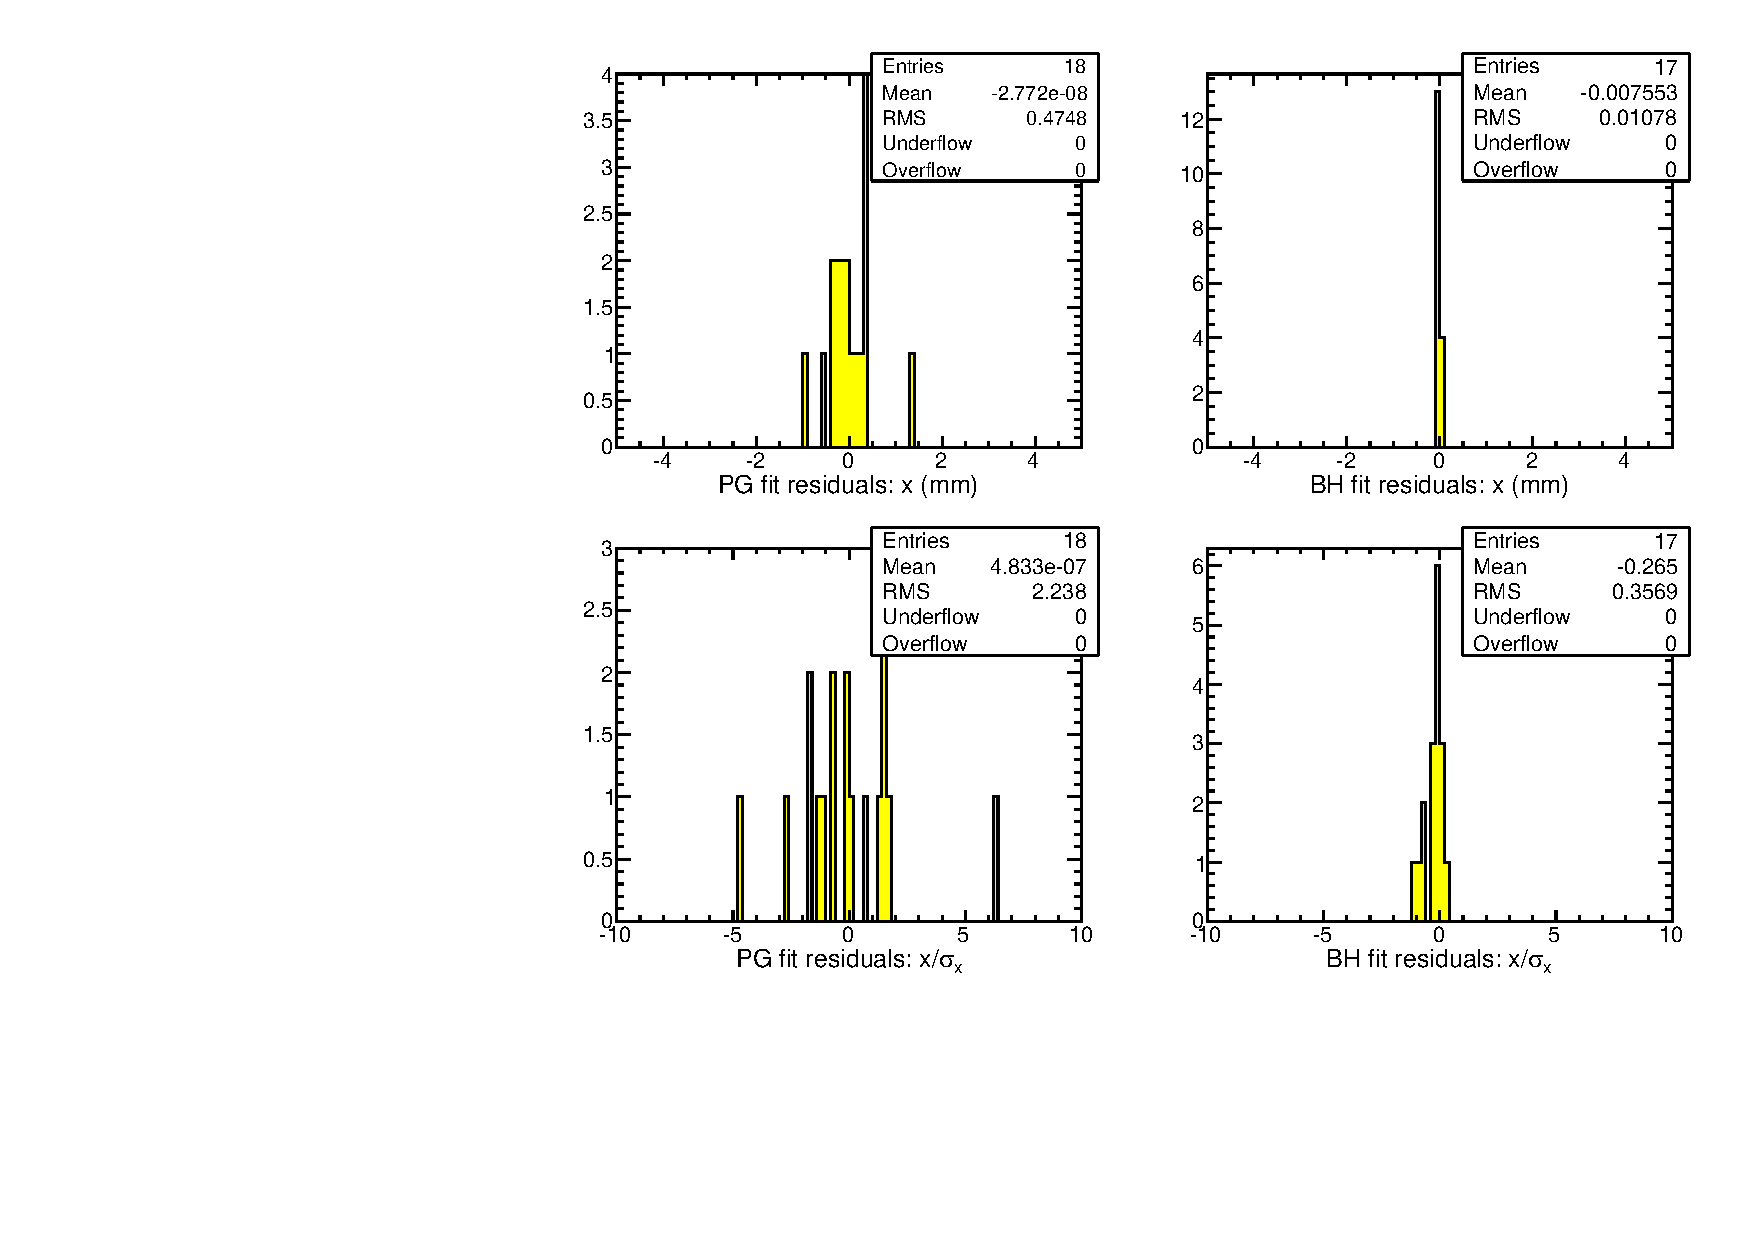
\includegraphics[width=\linewidth]{newplots_fitresiduals_MEp4_1_x.pdf}
\end{frame}
\begin{frame}
\frametitle{All results: ME$+$4/1 $\phi_z$}
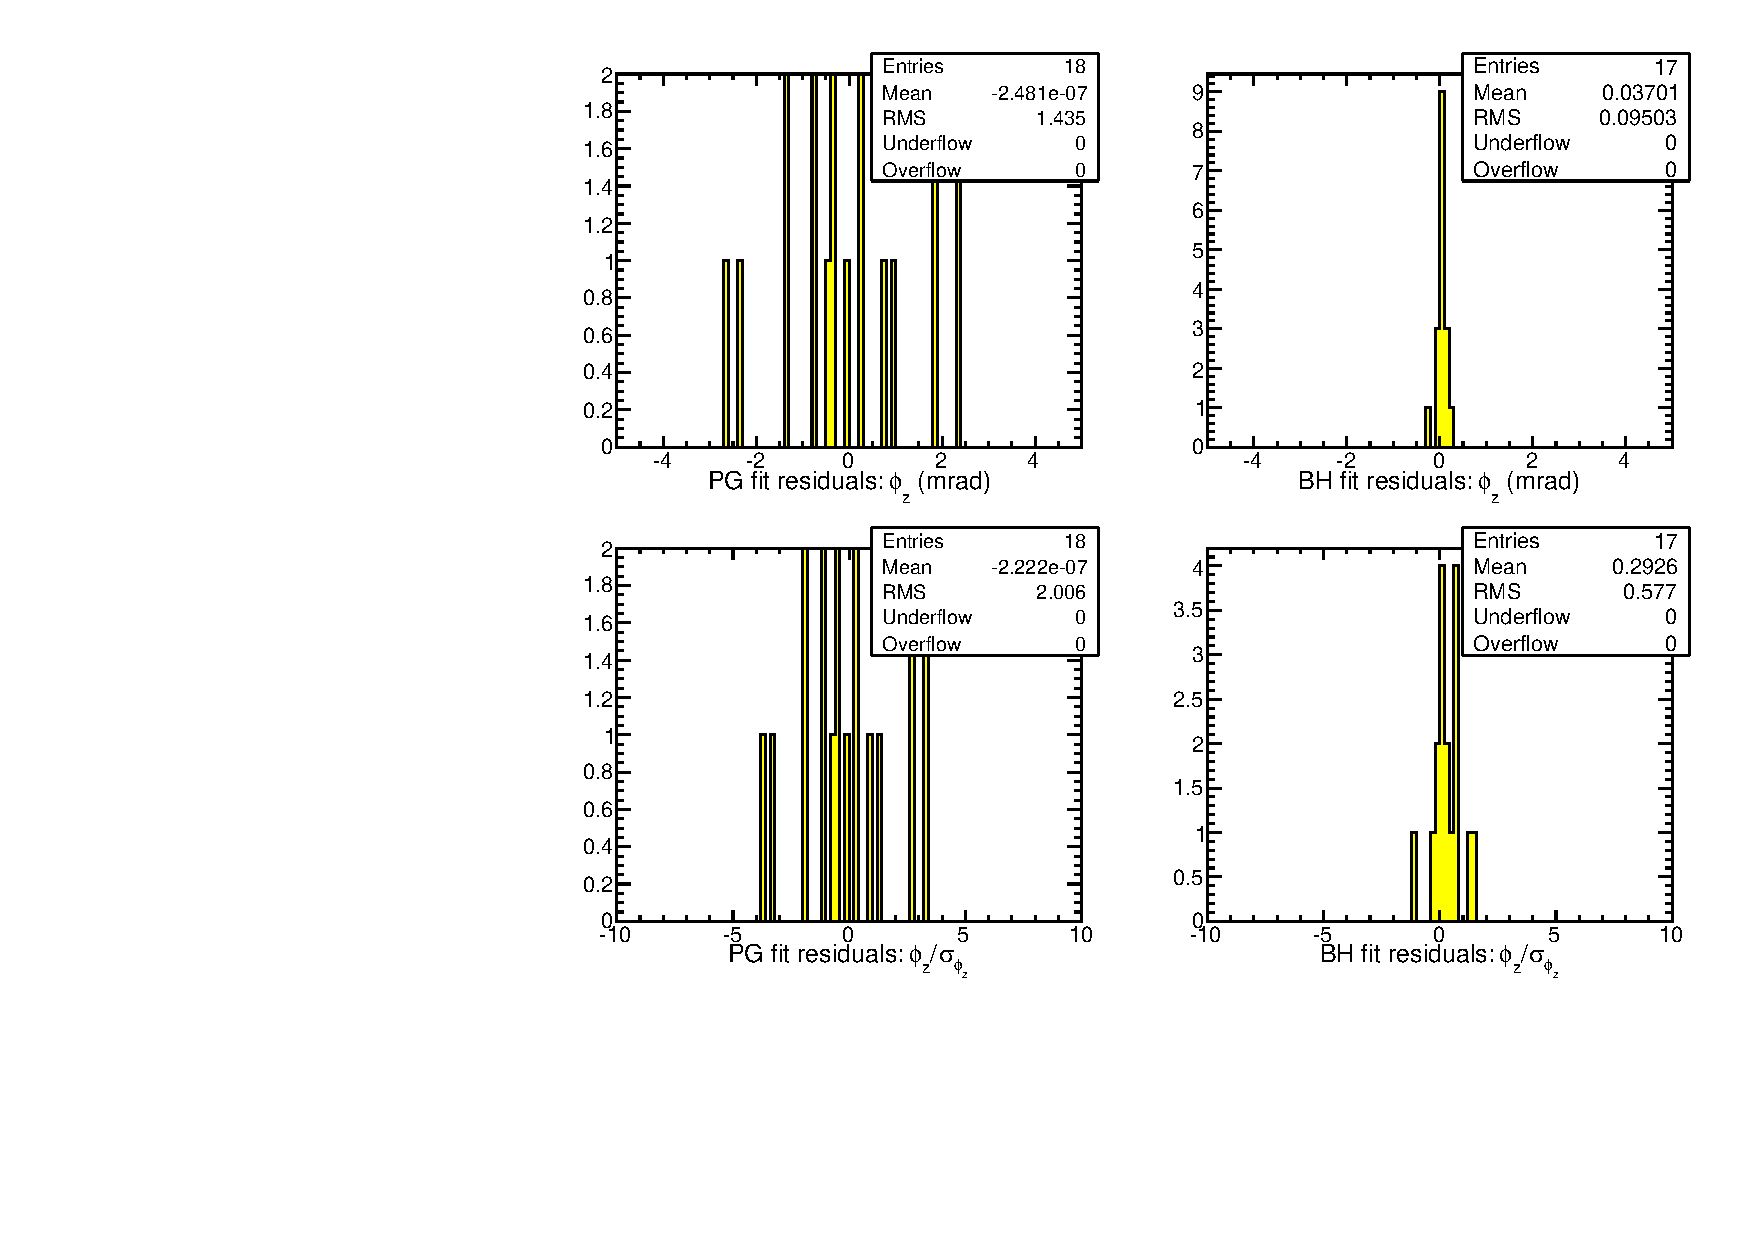
\includegraphics[width=\linewidth]{newplots_fitresiduals_MEp4_1_phiz.pdf}
\end{frame}

\begin{frame}
\frametitle{Future of ``other constraints''}
\begin{columns}
\column{0.6\linewidth}
\begin{itemize}
\item PG is consistent only at the level of 2$\sigma$ ($0.6\mbox{ mm} = 2\times 0.3\mbox{ mm}$)

\item We may be seeing a drift from 2007 to 2010, or with magnetic field

\item We can request a new PG with the next long shutdown, but we should also be able to use $r\phi$ and $\phi_z$ constraints from SLM lines

\item The fact that SLM lines only cover $\frac{1}{6}$ of chambers is okay because we only need it to fill the gaps in beam-halo data (as long as gaps in SLM and beam-halo data don't line up!)

\item Any topology and any constraint can be applied at the configuration file level.  We'd have to convert the SLM constraints into a \mbox{special text file format (not hard)\hspace{-5 cm}}
\end{itemize}

\column{0.4\linewidth}
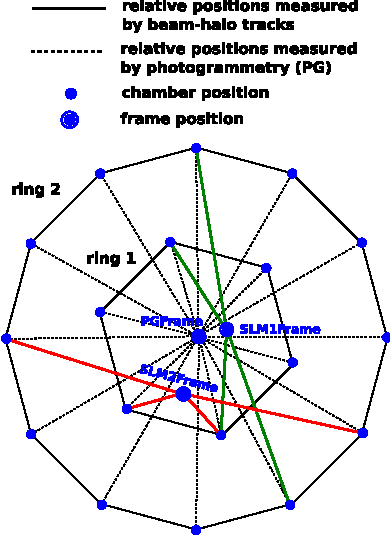
\includegraphics[width=\linewidth]{beamhalo-PG-SLM.pdf}
\end{columns}
\end{frame}

\begin{frame}
\frametitle{Ring radius correction}
\begin{itemize}
\item \textcolor{darkblue}{Why it's needed:} the value of $\sum_i m_{i,i+1}$ is unaffected
  by alignment, so if $\sum_i m_{i,i+1} \ne 0$, the pull is uniformly
  distributed around the ring:

\[ \mbox{pull}_{ij} = \frac{(m_{ij} - A_i + A_j)^2}{{\sigma_{ij}}^2} \]

\item Uncertainties $\sigma_{ij}$ vary by at least factors of 2, so in
  practice this means that only a few chambers absorb nearly all
  $\sum_i m_{i,i+1}$.

\end{itemize}

\begin{columns}
\column{0.5\linewidth}
A small error in radius $\displaystyle \Delta R = \frac{1}{2\pi} \sum_i m_{i,i+1}$, so $\Delta R \sim 1$~mm can mean introducing a $\mathcal{O}(6\mbox{ mm})$ error in the alignment, usually distributed like this:

\column{0.5\linewidth}
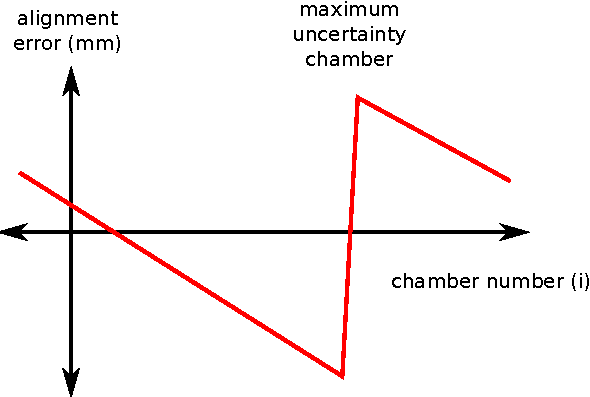
\includegraphics[width=\linewidth]{distribution_of_errors.pdf}
\end{columns}
\end{frame}

\begin{frame}
\frametitle{Ring radius correction}
\begin{itemize}
\item We can try to get the ring radius correction from sources
  outside of beam-halo alignment:
\begin{enumerate}
  \item Oleg measures bending of disks in magnetic field (from SLMs)
  \item Oleg gives me the lengths of posts (even and odd-numbered chambers)
  \item I put these angles and the implied ring-radius correction into the geometry
  \item I calculate $\sum_i m_{i,i+1}$ from the data using the new geometry
  \item I make an additional correction so that $\sum_i m_{i,i+1} \to 0$
\end{enumerate}

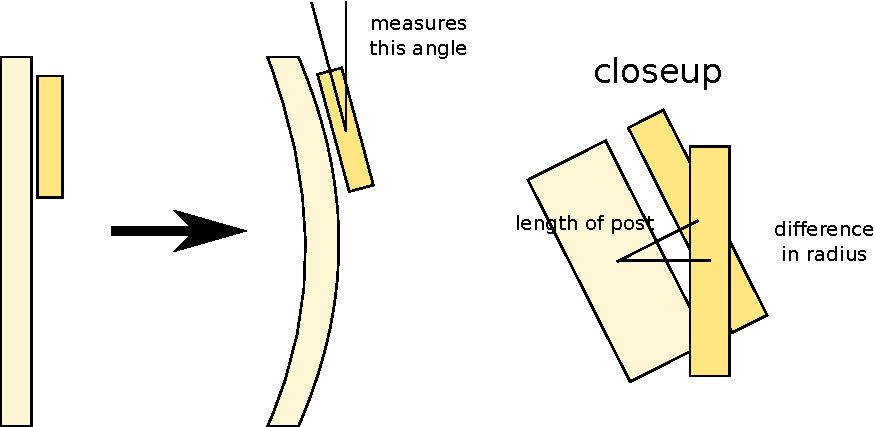
\includegraphics[width=0.9\linewidth]{ring_radius_correction.pdf}
\end{itemize}
\end{frame}

\begin{frame}
\frametitle{Ring radius correction}

Values of that ``additional correction'' (step 5)

\vfill
\renewcommand{\arraystretch}{1.3}
\begin{tabular}{r r p{1 cm} r r}
Ring & additional (mm) & & Ring & additional (mm) \\\hline
ME$+$1/2 &          $+$0.60 &&    ME$-$1/2 &          $+$0.11 \\
ME$+$2/1 &          $+$0.37 &&    ME$-$2/1 &          $+$0.04 \\
\textcolor{darkblue}{ME$+$2/2} &          \textcolor{darkblue}{$-$1.75} &&    ME$-$2/2 &          $-$0.79 \\
ME$+$3/1 &          $+$0.33 &&    ME$-$3/1 &          $-$0.11 \\
\textcolor{darkblue}{ME$+$3/2} &          \textcolor{darkblue}{$-$1.52} &&    \textcolor{darkblue}{ME$-$3/2} &          \textcolor{darkblue}{$-$1.56} \\
ME$+$4/1 &          $-$0.53 &&    ME$-$4/1 &          $-$0.55 \\
\end{tabular}
\end{frame}

%% \begin{frame}
%% \frametitle{Outline}
%% \begin{itemize}\setlength{\itemsep}{0.75 cm}
%% \item 
%% \end{itemize}
%% %% \hspace{-0.83 cm} \textcolor{darkblue}{\Large Outline2}
%% \end{frame}

%% \section*{First section}
%% \begin{frame}
%% \begin{center}
%% \Huge \textcolor{blue}{First section}
%% \end{center}
%% \end{frame}

\begin{frame}
\frametitle{Documentation}

\begin{itemize}
\item Gradually being filled in:

{\tiny \tt http://hepr8.physics.tamu.edu/pivarski/talks/alignment\_tutorial/alignment\_tutorial.pdf}

\item Beam-halo alignment touches on all aspects of alignment in a
  pedagogical way (each of the issues can be treated individually, not
  all at once)

\item So I'm writing this as a general alignment tutorial, but
  starting with the aspects which are particular to beam-halo alignment

\item Intended audience: {\it any} new graduate student--- I'm trying
  to encapsulate my expertise in this document

\item Includes working toy MC examples that I used to build my own intuition (quick little scripts)

\end{itemize}
\end{frame}

\begin{frame}
\frametitle{Documentation}

\begin{itemize}
\item \textcolor{darkblue}{Chapter 1: Introduction} \textcolor{red}{(done)}

\item \textcolor{darkblue}{Chapter 2: Propagating Alignment Measurements} \textcolor{red}{(almost done)}

\begin{minipage}{\linewidth}
\tiny Combining alignment measurements into a consistent system:
motivating examples, solution space is not $R^N$, logic and formalism
of simultaneous fitting with "constraint diagrams", Hessian, and
working toy example scripts.  Overconstrained systems and closure
tests.  Error analysis: decomposition of statistical errors into weak
and strong modes, characterization of the undetermined and weakest
modes, systematic errors in measurements.
\end{minipage}

\item \textcolor{darkblue}{Chapter 3: Measuring Detector Positions with Tracks}

\begin{minipage}{\linewidth}
\tiny Alignment measurements from tracks: 6-DOF rigid body parameter
space, track residuals space including the 4 relevant track
parameters, and the differential map (2dresid, 3doflargestruct,
6dof, 5dof, 6dofrphi) between them (linearization and iteration),
significance of the chamber origin, simple studies using elements
of the map, example from CRUZET alignment, toy example in pyROOT
(linear fit to plot and transformed residuals), full
track-parameter/alignment-parameter correlations and their
solutions: large-scale iteration and Millepede, Reference-Target
factorization of the problem.
\end{minipage}

\item \textcolor{darkblue}{Chapter 4: Realistic Tracking and Diagnostics of Track-Bias}

\begin{minipage}{\linewidth}
\tiny Systematic errors in realistic tracking: magnetic field errors,
material budget errors, and the q/pT, q/pz plots, Rutherford and
multiple scattering, argument for fitting to the peak, rather than
mean (CRUZET example), extension of the objective function and
non-linear minimization (PyMinuit example), cross-checks of
redundant constraints in the differential map, diagnosing track
biases: discontinuities at chamber boundaries (map plots),
differences of residuals on the same track (segment-difference
plots), and scaling of phi, theta, and curvature bias scaling with
pathlength.
\end{minipage}

\item \textcolor{darkblue}{Chapter 5: CSCOverlapsAlignmentAlgorithm: a Complete Alignment Package}

\begin{minipage}{\linewidth}
\tiny Technical details of the software package; layout of classes, built-in diagnostics, etc.
\end{minipage}

\item \textcolor{darkblue}{Chapter 6: Concluding Remarks}
\end{itemize}

\label{numpages}
\end{frame}

\end{document}
